%─────Lecture 1──────────────────────────────────────────────────────────────────────────────────────────────────────────────────────────────────────
\chapter{Introduction}
\marginpar{\footnotesize\textsf{\raggedright Lecture 1\\ September 10, 2026}}

\source{Slides pp.~2--3}

\begin{flushright}
	\itshape You must go into finance, Amory.\\
	\upshape --- F.~Scott Fitzgerald (1896--1940),\\
	\itshape This Side of Paradise\upshape\ (1920)

	\medskip

	\itshape The two most dangerous words in Wall Street\\
	vocabulary are ``financial engineering.''\\
	\upshape --- Wilbur Ross (2007)
\end{flushright}

\bigskip

\noindent The two epigraphs above already frame the tension this course lives in.
Finance is where quantitative modelling pays off most visibly, and it is also where a misplaced faith in a model does the most damage.
Our job is to learn the models \emph{and} to keep track of what they assume.

%─────§1 Class information───────────────────────────────────────────────────────────────────────────────────────────────────────────────────────────
\section{Class Information}

\source{Slides pp.~4--6}

The course follows the instructor's own textbook, and everything administrative lives on the course web page rather than in these notes.

\begin{itemize}[itemsep=0.35em]
	\item \textbf{Textbook.} Yuh-Dauh Lyuu, \emph{Financial Engineering \& Computation: Principles, Mathematics, Algorithms}.
	      Cambridge University Press, 2002.

	\item \textbf{Official web page.}
	      \begin{center}
		      \url{www.csie.ntu.edu.tw/~lyuu/finance1.html}
	      \end{center}
	      \begin{itemize}[nosep]
		      \item Lecture notes will be uploaded \emph{before} class.
		      \item Homeworks and teaching assistants will also be announced there.
		      \item Do not mistake last year's homeworks for this year's!
	      \end{itemize}

	\item \textbf{Software.} Some of the software used in the course is collected at
	      \begin{center}
		      \url{www.csie.ntu.edu.tw/~lyuu/capitals.html}
	      \end{center}

	\item \textbf{Questions.} Please ask many questions in class.
	      In a large class this is the best way for the instructor to remember you.\footnote{``[A] science concentrator [\ldots] said that in his eighth semester of [Harvard] college, there was not a single science professor who could identify him by name.'' (\emph{New York Times}, September 3, 2003.)}
\end{itemize}

%─────§2 Grading─────────────────────────────────────────────────────────────────────────────────────────────────────────────────────────────────────
\section{Grading}

\source{Slides p.~7}

Assessment is by \vocab{programming assignments} plus \vocab{one test}.
Every homework is to be treated as an examination, so the academic-integrity rules are strict:

\begin{itemize}[nosep]
	\item You are expected to write your own codes and to turn in your source code.
	\item Do not copy or collaborate with fellow students.
	\item Never ask your friends to write programs for you.
	\item Do not ask AI to code for you.
	\item Never give your codes to other students or publish your codes.
\end{itemize}

%─────§3 Scope──────────────────────────────────────────────────────────────────────────────────────────────────────────────────────────────────────
\section{Scope of the Course}

\source{Slides pp.~8--9}

\subsection{What This Course Is About}

The course runs from financial theory down to running code, in roughly this order:

\begin{itemize}[nosep]
	\item Financial theories in pricing.
	\item Mathematical backgrounds.
	\item Derivative securities.
	\item Pricing models.
	\item Efficient algorithms in pricing financial instruments.
	\item Research problems.
	\item Help in finding your thesis directions.
\end{itemize}

The last two items are worth emphasising: pricing problems that are merely ``computable'' are usually not good enough, and the gap between a correct algorithm and a \emph{fast} one is exactly where the open research questions sit.

\subsection{What This Course Is \texorpdfstring{\emph{Not}}{Not} About}

Equally important is what will \emph{not} be covered.

\begin{itemize}[itemsep=0.35em]
	\item \textbf{How to program.}\footnote{See \url{http://www.csie.ntu.edu.tw/train/}.} Programming ability is assumed, not taught --- but it matters.
	      A software bug cost Knight Capital Group, Inc.\ US\$457.6 million on August 1, 2012.\footnote{Kirilenko \& Lo (2013).}
	\item \textbf{Basic calculus, probability, combinatorics, and algebra.}
	\item \textbf{Details of the financial markets.}
	\item \textbf{How to be rich.}
	\item \textbf{How the markets will perform tomorrow.}
	\item \textbf{Professional behavior.}
\end{itemize}

\begin{moral}
	Pricing theory tells you what a security is worth \emph{given} a model of the market.
	It does not tell you what the market will do next.
\end{moral}

%─────§4 Journals───────────────────────────────────────────────────────────────────────────────────────────────────────────────────────────────────
\section{Useful Journals}

\source{Slides pp.~10--13}

The literature of the field is spread across finance, mathematics, operations research and computer science journals.
The following list is the one given in class.

\begin{multicols}{2}
	\begin{itemize}[nosep, font=\normalfont, label=\textcolor{Gray}{\textbullet}]
		\item \emph{Applied Mathematical Finance.}
		\item \emph{Applied Mathematics and Computations.}
		\item \emph{Communications on Pure and Applied Mathematics.}
		\item \emph{Computers \& Mathematics with Applications.}
		\item \emph{European Journal of Finance.}
		\item \emph{European Journal of Operational Research.}
		\item \emph{Finance and Stochastics.}
		\item \emph{Finance Research Letters.}
		\item \emph{Financial Analysts Journal.}
		\item \emph{Financial Management.}
		\item \emph{Insurance: Mathematics and Economics.}
		\item \emph{International Journal of Finance \& Economics.}
		\item \emph{International Journal of Theoretical and Applied Finance.}
		\item \emph{Journal of Banking \& Finance.}
		\item \emph{Journal of Computational Finance.}
		\item \emph{Journal of Derivatives.}
		\item \emph{Journal of Economic Dynamics \& Control.}
		\item \emph{Journal of Empirical Finance.}
		\item \emph{Journal of Finance.}
		\item \emph{Journal of Financial Economics.}
		\item \emph{Journal of Financial Markets.}
		\item \emph{Journal of Fixed Income.}
		\item \emph{Journal of Futures Markets.}
		\item \emph{Journal of Financial and Quantitative Analysis.}
		\item \emph{Journal of Portfolio Management.}
		\item \emph{Journal of Real Estate Finance and Economics.}
		\item \emph{Journal of Risk and Uncertainty.}
		\item \emph{Management Science.}
		\item \emph{Mathematical Finance.}
		\item \emph{Quantitative Finance.}
		\item \emph{Review of Financial Studies.}
		\item \emph{Review of Derivatives Research.}
		\item \emph{Review of Finance.}
		\item \emph{Risk Magazine.}
		\item \emph{SIAM Journal on Financial Mathematics.}
		\item \emph{Stochastics and Stochastics Reports.}
	\end{itemize}
\end{multicols}

%─────§5 Oath───────────────────────────────────────────────────────────────────────────────────────────────────────────────────────────────────────
\section{The Modelers' Hippocratic Oath}

\source{Slides p.~14}

Before writing down a single model, it is worth reading the oath proposed by Emanuel Derman and Paul Wilmott on January 7, 2009, in the wake of the financial crisis.

\begin{quote}
	\begin{itemize}[itemsep=0.3em, leftmargin=1em]
		\item I will remember that I didn't make the world, and it doesn't satisfy my
		      equations.
		\item Though I will use models boldly to estimate value, I will not be overly
		      impressed by mathematics.
		\item I will never sacrifice reality for elegance without explaining why I have
		      done so.
		\item Nor will I give the people who use my model false comfort about its
		      accuracy. Instead, I will make explicit its assumptions and oversights.
		\item I understand that my work may have enormous effects on society and the
		      economy, many of them beyond my comprehension.
	\end{itemize}
\end{quote}

\begin{intuition}
	A model is a deliberate simplification.
	The discipline is not in believing it, but in knowing precisely \emph{where} it is wrong and \emph{how much} that costs.
\end{intuition}

%─────§6 Markets───────────────────────────────────────────────────────────────────────────────────────────────────────────────────────────────────
\section{A First Look at the Markets and the Data}

\source{Slides p.~15}

Two facts motivate everything that follows.
First, the markets we want to price in are enormous, so even small pricing errors translate into large amounts of money.
Second, the price series they produce have a very definite statistical shape, and any pricing model has to be compatible with it.

\subsection{Outstanding U.S. Debts}

The fixed-income market alone is measured in tens of trillions of dollars, and over the period below it roughly quadrupled.
Note in particular how the \vocab{mortgage-related} and \vocab{asset-backed} columns grow --- these are precisely the securities whose pricing requires the algorithmic machinery of this course.

\newcommand{\zhcell}[1]{{\scriptsize\textcolor{black!55}{#1}}}
\begin{table}[H]
	\centering
	\footnotesize
	\setlength{\tabcolsep}{4pt}
	\begin{tabular}{c rrrrrrr r}
		\toprule
		     &           &          & \multicolumn{1}{c}{Mortgage-} & \multicolumn{1}{c}{U.S.}
		     & \multicolumn{1}{c}{Fed} & \multicolumn{1}{c}{Money} & \multicolumn{1}{c}{Asset-} &          \\
		Year & Municipal & Treasury & \multicolumn{1}{c}{related} & \multicolumn{1}{c}{corporate}
		     & \multicolumn{1}{c}{agencies} & \multicolumn{1}{c}{market} & \multicolumn{1}{c}{backed} & Total \\
		\zhcell{年份} & \zhcell{市政債} & \zhcell{美國公債}
		     & \multicolumn{1}{c}{\zhcell{房貸相關}} & \multicolumn{1}{c}{\zhcell{公司債}}
		     & \multicolumn{1}{c}{\zhcell{聯邦機構債}} & \multicolumn{1}{c}{\zhcell{貨幣市場}}
		     & \multicolumn{1}{c}{\zhcell{資產擔保}} & \zhcell{總計} \\
		\midrule
		85   & 859.5     & 1,437.7  & 372.1                                                       & 776.5    & 293.9   & 847.0    & 0.9     & 4,587.6  \\
		86   & 920.4     & 1,619.0  & 534.4                                                       & 959.6    & 307.4   & 877.0    & 7.2     & 5,225.0  \\
		87   & 1,010.4   & 1,724.7  & 672.1                                                       & 1,074.9  & 341.4   & 979.8    & 12.9    & 5,816.2  \\
		88   & 1,082.3   & 1,821.3  & 772.4                                                       & 1,195.7  & 381.5   & 1,108.5  & 29.3    & 6,391.0  \\
		89   & 1,135.2   & 1,945.4  & 971.5                                                       & 1,292.5  & 411.8   & 1,192.3  & 51.3    & 7,000.0  \\
		90   & 1,184.4   & 2,195.8  & 1,333.4                                                     & 1,350.4  & 434.7   & 1,156.8  & 89.9    & 7,745.4  \\
		91   & 1,272.2   & 2,471.6  & 1,636.9                                                     & 1,454.7  & 442.8   & 1,054.3  & 129.9   & 8,462.4  \\
		92   & 1,302.8   & 2,754.1  & 1,937.0                                                     & 1,557.0  & 484.0   & 994.2    & 163.7   & 9,192.8  \\
		93   & 1,377.5   & 2,989.5  & 2,144.7                                                     & 1,674.7  & 570.7   & 971.8    & 199.9   & 9,928.8  \\
		94   & 1,341.7   & 3,126.0  & 2,251.6                                                     & 1,755.6  & 738.9   & 1,034.7  & 257.3   & 10,505.8 \\
		95   & 1,293.5   & 3,307.2  & 2,352.1                                                     & 1,937.5  & 844.6   & 1,177.3  & 316.3   & 11,228.5 \\
		96   & 1,296.0   & 3,459.7  & 2,486.1                                                     & 2,122.2  & 925.8   & 1,393.9  & 404.4   & 12,088.1 \\
		97   & 1,367.5   & 3,456.8  & 2,680.2                                                     & 2,346.3  & 1,022.6 & 1,692.8  & 535.8   & 13,102.0 \\
		98   & 1,464.3   & 3,355.5  & 2,955.2                                                     & 2,666.2  & 1,296.5 & 1,978.0  & 731.5   & 14,447.2 \\
		99   & 1,532.5   & 3,281.0  & 3,334.2                                                     & 3,022.9  & 1,616.5 & 2,338.2  & 900.8   & 16,026.4 \\
		00   & 1,567.8   & 2,966.9  & 3,564.7                                                     & 3,372.0  & 1,851.9 & 2,661.0  & 1,071.8 & 17,056.1 \\
		01   & 1,688.4   & 2,967.5  & 4,125.5                                                     & 3,817.4  & 2,143.0 & 2,542.4  & 1,281.1 & 18,565.3 \\
		02   & 1,783.8   & 3,204.9  & 4,704.9                                                     & 3,997.2  & 2,358.5 & 2,577.5  & 1,543.3 & 20,170.1 \\
		\bottomrule
	\end{tabular}
	\caption{Outstanding U.S.\ debts, in billions of U.S.\ dollars.}
	\label{tab:us-debts}
\end{table}

\subsection{The Global OTC Derivatives Market}

\source{Slides p.~16}

Over-the-counter derivatives grew even faster, by close to an order of magnitude between 2000 and the 2008 crisis, after which the notional outstanding plateaued and then declined as trades were compressed and cleared centrally.

\begin{remark}
	\vocab{衍生性商品}（derivative）是價值取決於某個標的（利率、匯率、股價、信用等）的合約。
	\vocab{場外交易}（over-the-counter, OTC）指買賣雙方私下議定、不經交易所撮合的交易，與合約標準化、由結算所集中結算的\vocab{交易所交易}相對。
	OTC 合約可客製化（金額、到期日、標的皆可議），代價是雙方直接承擔\vocab{對手方風險}；市場由少數大型銀行（dealer）造市，未平倉部位以利率交換（interest rate swap）為大宗。

	\autoref{fig:otc} 的縱軸為\vocab{名目本金}（notional amount）——僅是計算利息與收益的參考金額，並非真正易手的資金，故市場實際市值遠小於此。
	2008 年金融危機後，美國 Dodd--Frank 法與歐盟 EMIR 要求標準化的 OTC 商品（尤其信用違約交換 CDS 與利率交換）改採\vocab{中央結算}（central clearing），並藉\vocab{壓縮}（compression）沖銷互相抵銷的部位，名目餘額因而在 2013 年前後見頂並回落。
\end{remark}

\begin{figure}[H]
	\centering
	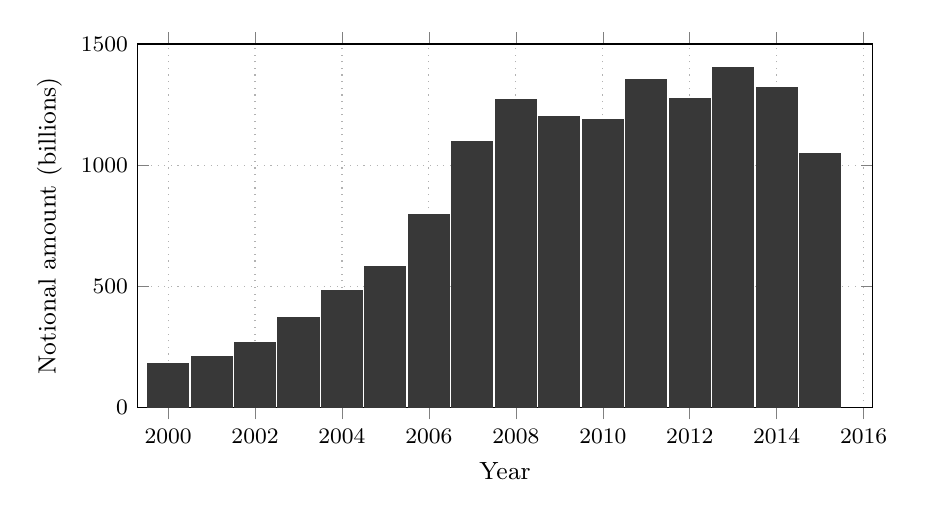
\begin{tikzpicture}
		\begin{axis}[
				width=0.9\textwidth, height=6.2cm,
				ybar, bar width=0.52cm,
				xmin=1999.3, xmax=2016.2,
				ymin=0, ymax=1500,
				xtick={2000,2002,2004,2006,2008,2010,2012,2014,2016},
				ytick={0,500,1000,1500},
				xlabel={Year},
				ylabel={Notional amount (billions)},
				tick label style={font=\footnotesize,
						/pgf/number format/1000 sep={}},
				label style={font=\small},
				grid=major, grid style={dotted, Gray!60},
				axis line style={thin},
			]
			\addplot[fill=black!78, draw=black!78] coordinates {
					(2000,180) (2001,212) (2002,268) (2003,370)
					(2004,482) (2005,582) (2006,795) (2007,1098)
					(2008,1272) (2009,1202) (2010,1188) (2011,1355)
					(2012,1276) (2013,1405) (2014,1320) (2015,1048)
				};
		\end{axis}
	\end{tikzpicture}
	\caption{The global OTC derivatives market. Bar heights are read off the
		chart shown in class.}
	\label{fig:otc}
\end{figure}

\subsection{The S\&P 500 Index and Its Returns}

\source{Slides pp.~17--19}

Robert Shiller\footnote{Co-winner of the 2013 Nobel Prize in Economic Sciences.} maintains a monthly series of the S\&P~500 index reaching back to 1871.
Plotted in levels (\autoref{fig:sp500}), it is dominated by the post-1980 growth; the 1929 crash is barely visible on this scale.

\begin{figure}[H]
	\centering
	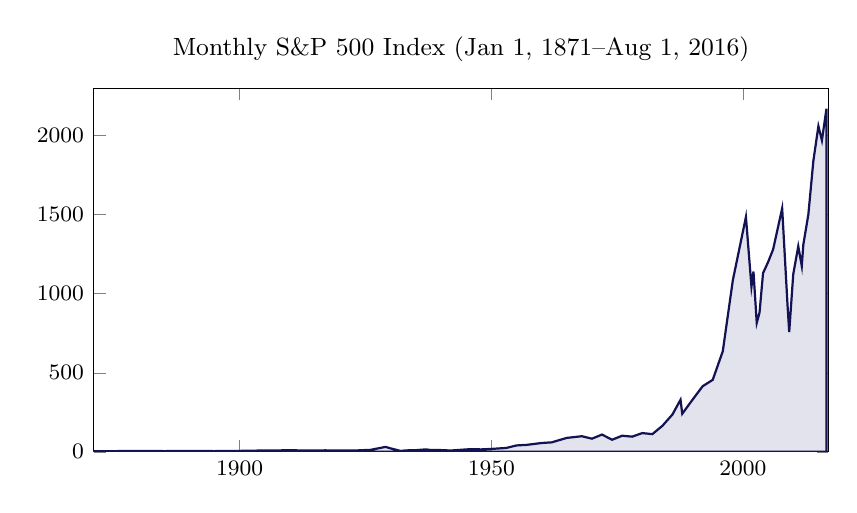
\begin{tikzpicture}
		\begin{axis}[
				width=0.9\textwidth, height=6.2cm,
				xmin=1871, xmax=2017, ymin=0, ymax=2300,
				xtick={1900,1950,2000},
				ytick={0,500,1000,1500,2000},
				title={\small Monthly S\&P 500 Index (Jan 1, 1871--Aug 1, 2016)},
				tick label style={font=\footnotesize,
						/pgf/number format/1000 sep={}},
				axis line style={thin},
			]
			\addplot[MidnightBlue!75!black, thick, fill=MidnightBlue!12] coordinates {
					(1871,4.4) (1875,4.5) (1880,5.5) (1885,4.6) (1890,5.3)
					(1895,4.6) (1900,6.1) (1905,8.6) (1910,9.8) (1915,8.3)
					(1917,9.5) (1920,7.8) (1923,8.6) (1926,12.6) (1929,31.3)
					(1930,21.7) (1931,13.7) (1932,5.5) (1933,9.1) (1935,10.6)
					(1937,15.4) (1938,11.5) (1940,11.0) (1942,8.4) (1945,15.2)
					(1946,17.1) (1948,15.5) (1950,18.4) (1953,24.7) (1955,40.5)
					(1957,44.0) (1960,55.9) (1962,60.0) (1965,88.2) (1968,98.7)
					(1970,83.2) (1972,109.2) (1974,76.5) (1976,102.0) (1978,96.1)
					(1980,118.7) (1982,111.9) (1984,164.5) (1986,236.3)
					(1987.6,329.4) (1987.95,240.9) (1990,330.2) (1992,415.0)
					(1994,455.2) (1996,636.0) (1998,1085.5) (2000.6,1485.5)
					(2001.7,1044.6) (2002.1,1140.0) (2002.75,815.3) (2003.3,880.0)
					(2004,1130.0) (2005,1200.0) (2006,1280.0) (2007.8,1540.0)
					(2008.9,910.0) (2009.2,757.1) (2010,1123.0) (2011,1300.0)
					(2011.7,1175.0) (2012,1310.0) (2013,1500.0) (2014,1840.0)
					(2015,2060.0) (2015.7,1970.0) (2016.6,2170.0)
				} \closedcycle;
		\end{axis}
	\end{tikzpicture}
	\caption{The S\&P 500 index in levels, reconstructed from the Shiller series.}
	\label{fig:sp500}
\end{figure}

Levels are not what we model, however.
Prices are non-stationary and their scale is arbitrary, so we work with the \vocab{log return} over one period,
\[
	r_t \;=\; \ln \frac{S_t}{S_{t-1}},
\]
where $S_t$ is the index level at time $t$.
\autoref{fig:sp500-returns} plots the monthly log returns of the same series.

\begin{remark}
	為什麼不直接對價位建模？
	\textbf{價位}（levels）是\vocab{非定態}的——統計性質隨時間漂移，1900 年與 2000 年的「正常水準」天差地遠，無法用一組固定參數描述；而且指數從幾點起編是人為選擇，尺度本身沒有經濟意義。
	改用\vocab{對數報酬} $r_t=\ln(S_t/S_{t-1})$ 一次補齊三件事：
	\begin{itemize}[nosep]
		\item $S_t/S_{t-1}$ 是本期的成長倍數（漲 2\% 即 $1.02$）。
		      變化小時 $\ln(1+x)\approx x$，所以 $r_t$ 近似百分比變化，且與絕對點數無關。
		\item \textbf{可加性}：跨期報酬 $\ln(S_t/S_{t-k})=r_t+r_{t-1}+\dots+r_{t-k+1}$，相加即可，不必連乘。
		\item 報酬率序列大致\textbf{定態}——繞著 0 波動、沒有趨勢，正適合建模。
	\end{itemize}
\end{remark}

\begin{figure}[H]
	\centering
	\pgfmathsetseed{20260910}
	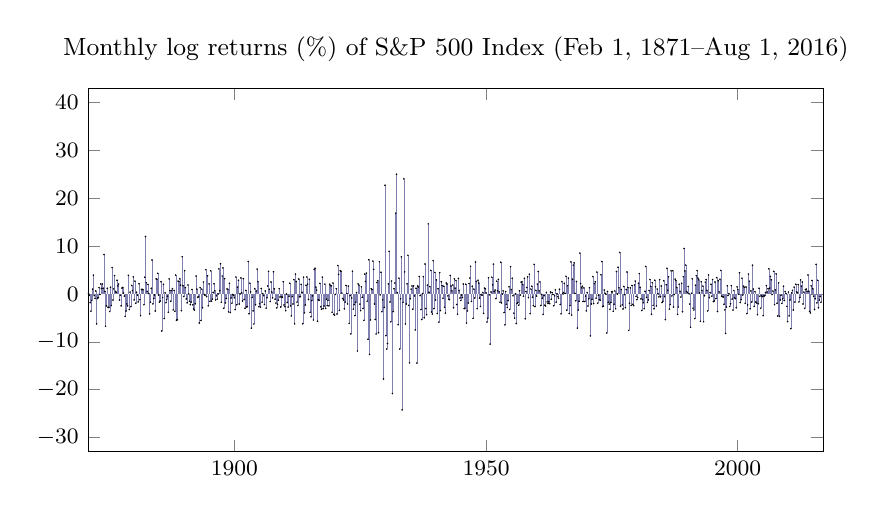
\begin{tikzpicture}
		\begin{axis}[
				width=0.9\textwidth, height=6.2cm,
				xmin=1871, xmax=2017, ymin=-33, ymax=43,
				xtick={1900,1950,2000},
				ytick={-30,-20,-10,0,10,20,30,40},
				title={\small Monthly log returns (\%) of S\&P 500 Index (Feb 1, 1871--Aug 1, 2016)},
				tick label style={font=\footnotesize,
						/pgf/number format/1000 sep={}},
				axis line style={thin},
			]
			\addplot[
				ycomb, MidnightBlue!55, line width=0.12pt,
				mark=*, mark size=0.22pt,
				mark options={draw=black, fill=black},
				domain=1871:2016.6, samples=900,
			]
			{3.6*rand + 10*rand*rand*rand
				+ 30*rand*rand/(1 + (x-1932)*(x-1932)/25)};
		\end{axis}
	\end{tikzpicture}
	\caption{Monthly log returns of the S\&P 500 index. The series is a
		schematic reproduction of the plot shown in class: it reproduces the mean,
		the typical amplitude, the fat tails and the volatility cluster of the early
		1930s, not the individual monthly observations.}
	\label{fig:sp500-returns}
\end{figure}

Three features stand out, and they will constrain every model we build:

\begin{itemize}[nosep]
	\item The returns hover around zero and show no obvious trend, in sharp contrast with the levels.
	\item Their amplitude is \emph{not} constant: quiet stretches alternate with violent ones (\vocab{volatility clustering}), the early 1930s being the extreme case.
	\item Large moves are far more frequent than a normal distribution would allow.
\end{itemize}

The last point is easiest to see from the empirical density (\autoref{fig:sp500-density}): the body is a sharp peak near zero, but the tails stay noticeably above zero out to $\pm 30\%$.

\begin{remark}
	兩個關鍵術語：\vocab{波動聚集}（volatility clustering）指抖動的\textbf{幅度}會成群出現——大波動旁邊通常還是大波動，平靜期也連成一片（1930 年代初最極端），也就是說波動率本身不是常數。
	\vocab{厚尾}（fat tails）指極端漲跌遠比常態分佈預測的頻繁。
	看\autoref{fig:sp500-density}：曲線畫的是每月報酬率的出現頻率，中央為 0 附近又高又尖的峰（多數月份幾乎不動），但兩側尾巴延伸到 $\pm 30\%$ 仍明顯高於零，而常態分佈在那裡的機率早已可忽略。
	這種「尖峰厚尾」的形狀，正是接下來那句結論的依據。
\end{remark}

\begin{figure}[H]
	\centering
	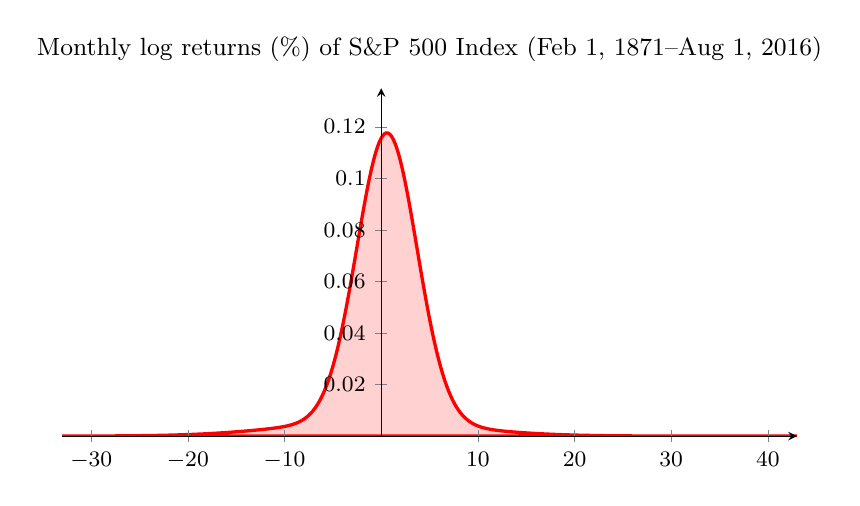
\begin{tikzpicture}
		\begin{axis}[
				width=0.9\textwidth, height=6.0cm,
				xmin=-33, xmax=43, ymin=0, ymax=0.135,
				xtick={-30,-20,-10,0,10,20,30,40},
				ytick={0.02,0.04,0.06,0.08,0.10,0.12},
				yticklabel style={/pgf/number format/fixed,
						/pgf/number format/precision=2},
				title={\small Monthly log returns (\%) of S\&P 500 Index (Feb 1, 1871--Aug 1, 2016)},
				tick label style={font=\footnotesize,
						/pgf/number format/1000 sep={}},
				axis x line=middle, axis y line=middle,
				axis on top,
				axis line style={thin},
			]
			\addplot[
				red, very thick, fill=red!18,
				domain=-33:43, samples=400,
			]
			{0.87*exp(0-(x-0.6)*(x-0.6)/19.22)/7.772
				+ 0.13*exp(0-(x+0.8)*(x+0.8)/162)/22.56}
			\closedcycle;
		\end{axis}
	\end{tikzpicture}
	\caption{Distribution of the monthly log returns of the S\&P 500 index:
		a sharp central peak with tails much heavier than the normal.}
	\label{fig:sp500-density}
\end{figure}

\begin{moral}
	Prices are not normally distributed, and their volatility is not constant.
	Any model that assumes otherwise is buying tractability with realism.

	價格並非常態分佈，波動率也非定值；凡是假設相反的模型，都是以寫實性為代價，換取數學上的易處理性。
\end{moral}

%─────§7 Analysis of algorithms────────────────────────────────────────────────────────────────────────────────────────────────────────────────────
\section{Analysis of Algorithms}

\source{Slides pp.~20--21}

\begin{flushright}
	\itshape I can calculate the motions\\
	of the heavenly bodies,\\
	but not the madness of people.\\
	\upshape --- Isaac Newton (1642--1727)

	\medskip

	\itshape It is unworthy of excellent men\\
	to lose hours like slaves\\
	in the labor of computation.\\
	\upshape --- Gottfried Wilhelm Leibniz (1646--1716)
\end{flushright}

\bigskip

\noindent Having seen how large the markets are and how awkward their data is, we now fix the vocabulary for the other half of the course: what it means for a pricing problem to be solvable, and at what cost.

\subsection{Computability and Algorithms}

\source{Slides p.~22}

\begin{definition}
	An \vocab{algorithm} is a precise procedure that can be turned into a computer program.
\end{definition}

Not every question admits one.
\vocab{Uncomputable} problems are those for which no algorithm exists at all, no matter how much time we are willing to spend.
Two standard examples --- both, uncomfortably, about programs themselves:

\begin{itemize}[nosep]
	\item Does this program have infinite loops?
	\item Is this program bug free?
\end{itemize}

Everything else is \vocab{computable}, and computable problems split again according to how expensive the algorithm is: \vocab{intractable} problems admit algorithms in principle but not ones we can afford to run, while \vocab{tractable} problems admit algorithms that are practical at the sizes we care about.
\autoref{fig:computability} summarises the picture.

\begin{figure}[H]
	\centering
	\begin{tikzpicture}[font=\small]
		% All problems
		\draw[rounded corners=6pt, draw=Gray!70, fill=Gray!4]
		(0,0) rectangle (13,5.1);
		\node[anchor=north west, font=\footnotesize\bfseries\sffamily,
			text=Gray!60!black] at (0.18,5.0) {All problems};

		% Uncomputable
		\draw[rounded corners=5pt, draw=WildStrawberry!70, fill=WildStrawberry!7]
		(0.35,0.35) rectangle (6.15,4.35);
		\node[anchor=north west, font=\footnotesize\bfseries\sffamily,
			text=WildStrawberry!70!black] at (0.55,4.22) {Uncomputable};
		\node[anchor=north west, text width=5.2cm, align=left, font=\footnotesize]
		at (0.55,3.7)
		{No algorithm exists.
			\begin{itemize}[nosep, leftmargin=1.1em, topsep=2pt]
				\item Does this program have infinite loops?
				\item Is this program bug free?
			\end{itemize}};

		% Computable
		\draw[rounded corners=5pt, draw=SeaGreen!70, fill=SeaGreen!7]
		(6.85,0.35) rectangle (12.65,4.35);
		\node[anchor=north west, font=\footnotesize\bfseries\sffamily,
			text=SeaGreen!60!black] at (7.05,4.22) {Computable};

		% Intractable
		\draw[rounded corners=4pt, draw=RawSienna!70, fill=RawSienna!10]
		(7.15,2.25) rectangle (12.35,3.65);
		\node[anchor=north west, font=\footnotesize\bfseries\sffamily,
			text=RawSienna!80!black] at (7.32,3.53) {Intractable};
		\node[anchor=north west, text width=4.7cm, font=\footnotesize]
		at (7.32,3.12) {Solvable in principle, too slow in practice.};

		% Tractable
		\draw[rounded corners=4pt, draw=SeaGreen!80, fill=SeaGreen!20]
		(7.15,0.65) rectangle (12.35,2.05);
		\node[anchor=north west, font=\footnotesize\bfseries\sffamily,
			text=SeaGreen!60!black] at (7.32,1.93) {Tractable};
		\node[anchor=north west, text width=4.7cm, font=\footnotesize]
		at (7.32,1.52) {Solvable at the problem sizes we actually meet.};
	\end{tikzpicture}
	\caption{The classification of problems. This course lives almost entirely
		in the bottom-right box --- and much of the research effort consists of
		moving pricing problems into it.}
	\label{fig:computability}
\end{figure}

\begin{remark}
	The conventional formal criterion is how running time scales with the input size $n$.
	A problem is counted \emph{tractable} when it admits an algorithm of \emph{polynomial} time, $O(n^{k})$ for some fixed $k$, and \emph{intractable} when it admits none --- every algorithm needs superpolynomial time, in most cases exponential. The rationale is practical: a polynomial bound keeps the cost manageable as $n$ grows, whereas anything superpolynomial blows up.
\end{remark}

\subsection{Complexity}

\source{Slides p.~23}

To measure cost without committing to a machine or a language, we count operations rather than seconds.

\begin{definition}
	A set of basic operations --- $+$, $-$, $\times$, $/$, $\log$, $x^{y}$, $e^{x}$, \ldots{} --- are assumed to take one unit of time each.
	The total number of such operations performed is the total work done by an algorithm, its \vocab{computational complexity}.
	The amount of memory space it uses is its \vocab{space complexity}.
\end{definition}

\begin{remark}
	Two conventions are worth making explicit.
	\begin{itemize}[nosep]
		\item We concentrate on the \emph{abstract} complexity of an algorithm instead of its detailed implementation.
		      Constant factors from the language, compiler and hardware are deliberately ignored.
		\item Despite that, complexity is a good guide to an algorithm's \emph{actual} running time.
		      It is the coarse measure that survives a change of machine.
	\end{itemize}
\end{remark}

\subsection{Common (Asymptotic) Complexities}

\source{Slides p.~24}

Let $n$ stand for the ``size'' of the problem --- the number of elements, the number of cash flows, the number of time periods, and so on.
Complexity is then expressed as a function of $n$, and the standard names are as follows.

\begin{table}[H]
	\centering
	\begin{tabular}{@{}l l l@{}}
		\toprule
		Name             & Complexity          & Remark                                    \\
		\midrule
		Linear           & $O(n)$              &                                           \\
		Quadratic        & $O(n^{2})$          &                                           \\
		Cubic            & $O(n^{3})$          &                                           \\
		Superpolynomial  & e.g.\ $2^{O(\sqrt{n})}$
		                 & higher than any polynomial\footnotemark                         \\
		Exponential time & $2^{O(n)}$          & the usual worst case                      \\
		\bottomrule
	\end{tabular}
	\caption{Common asymptotic complexities, in increasing order of growth.}
	\label{tab:complexities}
\end{table}
\footnotetext{E.g., T.~Dai (\texttt{B82506025}, \texttt{R86526008}, \texttt{D8852600}) \& Lyuu (2007); Lyuu \& C.~Wang (\texttt{F95922018}) (2011); H.~Chiu (\texttt{R98723059}) (2012).}

\begin{note}
	The superpolynomial entry is not a curiosity.
	Several pricing problems that were only known to admit exponential-time algorithms have been pushed down to $2^{O(\sqrt{n})}$ --- an improvement large enough to turn an unusable algorithm into a usable one, and precisely the kind of result this course aims at.
\end{note}

%─────Basic Financial Mathematics────────────────────────────────────────────────────────────────────────────────────────────────────────────────────
\chapter{Basic Financial Mathematics}

\source{Slides pp.~25--26}

\begin{flushright}
	\itshape In the fifteenth century\\
	mathematics was mainly concerned with\\
	questions of commercial arithmetic and\\
	the problems of the architect.\\
	\upshape --- Joseph Alois Schumpeter (1883--1950)

	\medskip

	\itshape I'm more concerned about\\
	the return \emph{of} my money than\\
	the return \emph{on} my money.\\
	\upshape --- Will Rogers (1879--1935)
\end{flushright}

\bigskip

\noindent Everything in this chapter follows from one idea: a dollar today and a dollar next year are different goods, and the interest rate is the exchange rate between them.
Once that exchange rate is pinned down, valuing a stream of payments is arithmetic --- and, as we will see, arithmetic whose cost we can still argue about.

%─────§ The time line──────────────────────────────────────────────────────────────────────────────────────────────────────────────────────────────
\section{The Time Line}

\source{Slides p.~27}

Before any formula, fix the convention for talking about time.
Time is measured in \vocab{periods}; time~$0$ is now, and period~$k$ is the interval running from time $k-1$ to time~$k$.
A cash flow ``at time~$k$'' arrives at the \emph{end} of period~$k$.

\begin{figure}[H]
	\centering
	\begin{tikzpicture}[font=\small]
		\draw[-{Stealth[length=6pt]}] (-0.3,0) -- (11.6,0);
		\foreach \x/\lbl in {0/0, 2.6/1, 5.2/2, 7.8/3, 10.4/4} {
				\draw[thick] (\x,-0.12) -- (\x,0.42);
				\node[below=3pt] at (\x,-0.12) {Time \lbl};
			}
		\foreach \x/\lbl in {1.3/1, 3.9/2, 6.5/3, 9.1/4} {
				\node[above=2pt] at (\x,0.42) {Period \lbl};
			}
	\end{tikzpicture}
	\caption{The time line. Period~$k$ spans time $k-1$ to time~$k$.}
	\label{fig:timeline}
\end{figure}

%─────§ Time value of money───────────────────────────────────────────────────────────────────────────────────────────────────────────────────────
\section{Time Value of Money}

\source{Slides p.~28}

\begin{definition}
	Let $r$ be the \vocab{interest rate} per period.
	The \vocab{future value} (FV) and \vocab{present value} (PV) of a single amount over $n$ periods are related by
	\begin{align}
		\mathrm{FV} & = \mathrm{PV}(1+r)^{n}, \label{eq:fv-pv}         \\
		\mathrm{PV} & = \mathrm{FV} \times (1+r)^{-n}. \nonumber
	\end{align}
\end{definition}

\begin{intuition}
	$(1+r)^{n}$ carries money forward in time and $(1+r)^{-n}$ carries it backward.
	\emph{Discounting} --- the second operation --- is the one we use constantly, because a security's price is quoted today while its payoffs arrive later.

	$(1+r)^{n}$ 把錢往未來搬，$(1+r)^{-n}$ 把錢往現在搬。
	我們不斷用到的是後者—— \textbf{折現}（discounting）——因為證券的價格報在今天，收益卻在日後才到。
\end{intuition}

The idea is old: it goes back to Fibonacci (1170--1240), and was put on a modern footing by Irving Fisher (1867--1947).

%─────§ Compounding───────────────────────────────────────────────────────────────────────────────────────────────────────────────────────────────
\section{Compounding}

\source{Slides pp.~29--30}

Equation~\eqref{eq:fv-pv} is stated per \emph{period}, but rates are quoted per \emph{year}.
Reconciling the two is what compounding conventions are for --- and getting the convention wrong is a classic source of pricing errors.

\subsection{Periodic Compounding}

Suppose the \emph{annual} interest rate $r$ is compounded $m$ times per annum.
Each compounding period earns $r/m$, so one dollar grows along
\[
	1 \;\to\; \Bigl(1+\frac{r}{m}\Bigr)
	\;\to\; \Bigl(1+\frac{r}{m}\Bigr)^{2}
	\;\to\; \Bigl(1+\frac{r}{m}\Bigr)^{3}
	\;\to\; \cdots
\]
Hence, after $n$ years,
\begin{equation}
	\mathrm{FV} = \mathrm{PV}\Bigl(1+\frac{r}{m}\Bigr)^{nm}. \label{eq:periodic}
\end{equation}

\subsection{Common Compounding Methods}

\begin{center}
	\begin{tabular}{@{}ll@{\qquad}ll@{}}
		\toprule
		Method      & $m$ & Method                 & $m$      \\
		\midrule
		Annual      & 1   & Weekly                 & 52       \\
		Semiannual  & 2   & Daily                  & 365      \\
		Quarterly   & 4   & Continuous             & $\infty$ \\
		Monthly     & 12  &                        &          \\
		\bottomrule
	\end{tabular}
\end{center}

\subsection{Translating between Rate and Frequency}

\source{Slides pp.~31--32}

An annual interest rate of $r$ compounded $m$ times a year is ``equivalent to'' an interest rate of $r/m$ per $1/m$ year.
Read in reverse: if a loan asks for a return of $1\%$ \emph{per month}, the \emph{annual} interest rate will be $12\%$ with monthly compounding.

\begin{eg}
	The annual interest rate is $10\%$ compounded twice per annum.
	Each dollar will grow to be
	\[
		\bigl[\,1+(0.1/2)\,\bigr]^{2} = 1.1025
	\]
	one year from now.
	The rate is therefore ``equivalent to'' an interest rate of $10.25\%$ compounded once \emph{per annum}, since
	\[
		1 + 0.1025 = 1.1025 .
	\]
\end{eg}

The $10.25\%$ in the example is the \vocab{effective annual rate}: the single annually-compounded rate that produces the same money after one year.
The quoted $10\%$ is only a \vocab{nominal rate}, and by itself it does not determine anything.

\begin{moral}
	An interest rate is meaningless without the compounding frequency.
\end{moral}

\subsection{The Rule of 72}

\source{Slides pp.~33--35}

Let the annual interest rate be $r$ with annual compounding.
How many years $T$ will it take for your money to double?
The identity to solve is
\[
	(1+r)^{T} = 2,
	\qquad\text{so}\qquad
	T = \frac{\ln 2}{\ln (1+r)} .
\]
Is there an easier way?
The \vocab{rule of 72} is a heuristic that estimates $T$ without a logarithm:
\begin{equation}
	T \approx \frac{72}{r\ (\%)} . \label{eq:rule72}
\end{equation}
So it takes about $72/12 = 6$ years to double the GDP if the annual growth rate is $12\%$.

\begin{proof}[Reason]
	Expanding $\ln(1+r) = r - r^{2}/2 + O(r^{3})$ gives, for small $r$,
	\[
		\frac{1}{\ln(1+r)}
		\;\approx\; \frac{1}{r\,(1-r/2)}
		\;\approx\; \frac{1}{r} + \frac{1}{2},
	\]
	and therefore
	\[
		\frac{\ln 2}{\ln(1+r)} \;\approx\; \frac{0.693}{r} + 0.3466 . \qedhere
	\]
\end{proof}

\begin{remark}
	The leading constant is $0.693$, i.e.\ $69.3$ when $r$ is measured in percent --- so a ``rule of 69.3'' is the asymptotically correct one.
	The extra $+0.3466$ is a positive offset, so inflating the numerator to $72$ compensates for it over the range of rates one actually meets.
	That $72$ is also divisible by $2,3,4,6,8,9,12$ is a large part of why it, rather than $70$, became the folk rule.
\end{remark}

\autoref{fig:rule72} plots the error of both variants: the true interest rate minus the approximation, in percent, against the number of years to double.

\begin{remark}
	這張圖把 Eq.~\eqref{eq:rule72} \textbf{反過來用}：平常是「給利率 $r$，估翻倍要幾年 $T$」，這裡改成「給橫軸的 $T$（想要幾年翻倍），估需要多少利率」——把公式解成 $r\approx 72/T$。
	縱軸畫的是兩個\textbf{利率}估計值的差：真正在 $T$ 年翻倍所需的 $r_{\text{真}}=2^{1/T}-1$，減去 Rule of 72 反解出的 $r_{\text{估}}=72/T$（兩者都乘 $100$ 化成百分比）。
	所以縱軸單位是「利率的百分點」，不是「年」；橫軸的 $T$ 在這裡是已知條件，不是被估計的量。

	代入數字比較有感覺：$T=1$ 年時，真正利率 $100\%$ 對 Rule of 72 的 $72\%$，差 $28$ 個百分點，極不準；$T=8$ 年時，真正利率約 $9.05\%$ 對 $9\%$，差只有 $0.05$，正是 caption 說的「超過約 8 年後極準」；$T=20$ 年時差變成負的（約 $-0.07$），代表 Rule of 72 在長期會略為高估所需利率（``overshoot''）。
\end{remark}

\begin{figure}[H]
	\centering
	\begin{tikzpicture}
		\begin{groupplot}[
				group style={group size=2 by 1, horizontal sep=1.1cm,
						ylabels at=edge left},
				width=0.46\textwidth, height=5.2cm,
				xmin=0, xmax=20, ymin=-2, ymax=30,
				xtick={0,5,10,15,20},
				ytick={0,5,10,15,20,25,30},
				xlabel={Number of years to double},
				ylabel={Error in interest rate (\%)},
				label style={font=\footnotesize},
				tick label style={font=\footnotesize},
				axis line style={thin},
			]
			\nextgroupplot[title={\small Rule of 72}]
			\addplot[MidnightBlue!70, thick, mark=*, mark size=0.6pt,
				domain=1:20, samples=20] {100*(2^(1/x)-1) - 72/x};
			\nextgroupplot[title={\small Rule of 70}]
			\addplot[MidnightBlue!70, thick, mark=*, mark size=0.6pt,
				domain=1:20, samples=20] {100*(2^(1/x)-1) - 70/x};
		\end{groupplot}
	\end{tikzpicture}
	\caption{How good is the rule of 72? Plotted is the true interest rate
		minus the approximation (in \%). Both are badly off for very short
		doubling times and excellent beyond about eight years; the rule of 72
		slightly \emph{over}shoots there, the rule of 70 slightly undershoots.}
	\label{fig:rule72}
\end{figure}

\subsection{Continuous Compounding}

\source{Slides pp.~36--37}

Let $m \to \infty$ in Eq.~\eqref{eq:periodic}, so that
\[
	\Bigl(1+\frac{r}{m}\Bigr)^{m} \longrightarrow e^{r} .
\]
Then
\begin{equation}
	\mathrm{FV} = \mathrm{PV} \times e^{rn}, \label{eq:continuous}
\end{equation}
where $e = 2.71828\ldots$\ \footnote{Jacob Bernoulli (1654--1705) in 1685.}

Continuous compounding is easier to work with, because the exponents simply add.
Suppose the annual interest rate is $r_{1}$ for $n_{1}$ years and $r_{2}$ for the following $n_{2}$ years.
Then the FV of one dollar will be
\[
	e^{r_{1}n_{1} + r_{2}n_{2}}
\]
after $n_{1}+n_{2}$ years --- no nested products, just a sum in the exponent.

\subsection{Conversion between Compounding Methods}

\source{Slides pp.~38--40}

Let $r_{1}$ be the annual rate with continuous compounding and $r_{2}$ the \emph{equivalent} rate compounded $m$ times per annum.
How are they related?

\begin{proposition}
	The principle is that both interest rates must produce the same amount of money after one year, that is,
	\[
		\Bigl(1+\frac{r_{2}}{m}\Bigr)^{m} = e^{r_{1}} .
	\]
	Therefore\footnote{Are they really equivalent?
	In what sense are they equivalent?
	Contributed by Mr.~Chen, Tung-Li (\texttt{D09922014}) on February 24, 2023.}
	\begin{align*}
		r_{1} & = m \ln\Bigl(1+\frac{r_{2}}{m}\Bigr), \\
		r_{2} & = m\bigl(e^{r_{1}/m}-1\bigr).
	\end{align*}
\end{proposition}

The same principle handles two periodic conventions.
Suppose $r_{1}$ is the annual rate compounded $m_{1}$ times per annum and $r_{2}$ is the \emph{equivalent} rate compounded $m_{2}$ times per annum.
Then
\begin{equation}
	\Bigl(1+\frac{r_{1}}{m_{1}}\Bigr)^{m_{1}}
	= \Bigl(1+\frac{r_{2}}{m_{2}}\Bigr)^{m_{2}} . \label{eq:conversion}
\end{equation}

\begin{observation}
	Every conversion in this subsection is the same one-line demand: \emph{equal value after one year}.
	There is nothing to memorise beyond that.
\end{observation}

%─────§ Present value───────────────────────────────────────────────────────────────────────────────────────────────────────────────────────────────
\section{Present Value}

\source{Slides p.~41}

\subsection{The PV Formula}

\begin{definition}
	The PV of the cash flow $C_{1}, C_{2}, \ldots, C_{n}$ at times $1, 2, \ldots, n$ is
	\begin{equation}
		\mathrm{PV} = \frac{C_{1}}{1+y} + \frac{C_{2}}{(1+y)^{2}}
		+ \cdots + \frac{C_{n}}{(1+y)^{n}} , \label{eq:pv}
	\end{equation}
	where $y$ is the discount rate per period.
\end{definition}

\begin{remark}
	我們想要衡量一筆包含未來的錢的現金流折算到現在價值多少，這條公式就是把單筆折現 $\mathrm{PV}=\mathrm{FV}(1+y)^{-n}$ \textbf{對每一筆現金流各做一次，再加起來}：在 time $k$ 收到的 $C_{k}$ 要往回搬 $k$ 期，所以除以 $(1+y)^{k}$—— 越晚到的錢折得越兇——加總便是整串現金流今天的總值。
	$y$ 是每期折現率，字母取自 \emph{yield}，角色與前一章的 $r$ 相同。
\end{remark}

This formula and its variations are the engine behind most of financial calculations.\footnote{Cochrane (2005), ``Asset pricing theory all stems from one simple concept [\ldots]: price equals expected discounted payoff.''} The difficulty is never the algebra; it is deciding what goes into it:

\begin{itemize}[nosep]
	\item What is $y$?
	\item What are the $C_{i}$?
	\item What is $n$?
\end{itemize}

\begin{note}
	Equation~\eqref{eq:pv} is taken on faith for now.
	It will be justified later in the course from ``sound'' principles rather than assumed.
\end{note}

\subsection{Evaluating the PV Formula}

\source{Slides pp.~42--44}

Even a formula this simple raises the question the previous chapter set up: how much work does it actually take?
The direct transcription is \autoref{alg:pv-direct}.

\begin{algorithm}[H]
	\caption{Evaluating the PV in Eq.~\eqref{eq:pv} directly}
	\label{alg:pv-direct}
	$x := 0$\;
	\For{$i = 1, 2, \ldots, n$}{
		$x := x + C_{i}/(1+y)^{i}$\;
	}
	\Return{$x$}\;
\end{algorithm}

Computing $(1+y)^{i}$ by repeated multiplication costs $i$ operations, so the algorithm takes time proportional to $\sum_{i=1}^{n} i = O(n^{2})$ if only $+,-,\times$ and $/$ are allowed.
It can be improved to $O(n)$ by applying $a^{b} = e^{b\ln a}$ in step~3, since we agreed to count $x^{y}$ as taking one unit of time.

But there is a better route, which needs no exponentiation at all (\autoref{alg:pv-horner}).

\begin{algorithm}[H]
	\caption{Evaluating the PV by Horner's rule}
	\label{alg:pv-horner}
	$x := 0$\;
	$d := 1+y$\;
	\For{$i = n, n-1, \ldots, 1$}{
		$x := (x + C_{i})/d$\;
	}
	\Return{$x$}\;
\end{algorithm}

\begin{proposition}[Horner's rule]
	The underlying identity is
	\[
		\Biggl(\cdots\biggl(\Bigl(\frac{C_{n}}{1+y}+C_{n-1}\Bigr)\frac{1}{1+y}
		+ C_{n-2}\biggr)\frac{1}{1+y} + \cdots\Biggr)\frac{1}{1+y} ,
	\]
	due to Horner (1786--1837) in 1819.
\end{proposition}

The algorithm takes $O(n)$ time, and it is the most efficient possible in terms of the absolute number of arithmetic operations.\footnote{A.~Borodin \& Munro (1975).} It can also be computed in parallel in $O(\log n)$ time using prefix sums.\footnote{Contributed by Mr.~Chen, Yi-Feng (\texttt{R08922077}) on February 24, 2021.}

\begin{moral}
	Two algorithms for the same formula, $O(n^{2})$ against $O(n)$ --- and the fast one is also the numerically simpler one.
	This is the pattern the whole course chases.
\end{moral}

%─────§ Annuities────────────────────────────────────────────────────────────────────────────────────────────────────────────────────────────────────
\section{Annuities}

\source{Slides pp.~45--47}

\subsection{Annuities Certain}

\begin{definition}
	An \vocab{annuity} pays out the same $C$ dollars at the end of each year for $n$ years.
\end{definition}

\begin{figure}[H]
	\centering
	\begin{tikzpicture}[font=\small]
		\node[anchor=east] at (-0.6,0.45) {Cash flow:};
		\draw[-{Stealth[length=6pt]}] (-0.3,0) -- (9.6,0);
		\foreach \x/\lbl in {1.7/1, 3.4/2, 5.1/3} {
				\draw[-{Stealth[length=5pt]}, thick] (\x,0) -- (\x,0.75);
				\node[above=1pt] at (\x,0.75) {$C$};
				\node[below=2pt] at (\x,0) {$\lbl$};
			}
		\node at (6.3,0.5) {$\cdots$};
		\draw[-{Stealth[length=5pt]}, thick] (7.5,0) -- (7.5,0.75);
		\node[above=1pt] at (7.5,0.75) {$C$};
		\node[below=2pt] at (7.5,0) {$n$};
	\end{tikzpicture}
	\caption{The cash flow of an $n$-year annuity certain.}
	\label{fig:annuity-cashflow}
\end{figure}

With a rate of $r$, specialising Eq.~\eqref{eq:pv} to $C_{i} \equiv C$ and summing the geometric series gives
\[
	\mathrm{PV} = \sum_{i=1}^{n} C(1+r)^{-i}
	= C\,\frac{1-(1+r)^{-n}}{r} ,
\]
while the FV at the end of the $n$th year is
\[
	\mathrm{FV} = \sum_{i=0}^{n-1} C(1+r)^{i}
	= C\,\frac{(1+r)^{n}-1}{r} .
\]
The study of these sums goes back to Jan de Witt (1625--1672) in 1671 and Nicholas Bernoulli (1687--1759) in 1709.

\subsection{General Annuities}

Suppose instead that $m$ payments of $C$ dollars each are received per year (the \vocab{general annuity}), and let $r$ be compounded $m$ times per annum.\footnote{If your $r$ has a compounding frequency different from $m$, convert it with Eq.~\eqref{eq:conversion} first.} Then the same geometric sum with period rate $r/m$ and $nm$ periods gives
\begin{align}
	\mathrm{PV} & = \sum_{i=1}^{nm} C\Bigl(1+\frac{r}{m}\Bigr)^{-i}
	= C\,\frac{1-\bigl(1+\frac{r}{m}\bigr)^{-nm}}{\frac{r}{m}},
	\label{eq:gen-annuity}                                             \\
	\mathrm{FV} & = \sum_{i=0}^{nm-1} C\Bigl(1+\frac{r}{m}\Bigr)^{i}
	= C\,\frac{\bigl(1+\frac{r}{m}\bigr)^{nm}-1}{\frac{r}{m}} . \nonumber
\end{align}

\begin{remark}
    Annuity is paid at the end of every year, so note the indices of above formulas.
\end{remark}

%─────§ Amortization──────────────────────────────────────────────────────────────────────────────────────────────────────────────────────────────
\section{Amortization}

\source{Slides pp.~48--49}

\subsection{The Amortization Method}

\begin{definition}
	\vocab{Amortization} is a method of repaying a loan through regular payments of interest \emph{and} principal.
\end{definition}

The mechanics are worth stating carefully, because every line of the schedule below follows from them:

\begin{itemize}[nosep]
	\item The size of the loan (the original balance) is reduced by the \emph{principal} part of each payment.
	\item The \emph{interest} part of each payment pays the interest incurred on the \emph{remaining} principal balance.
	\item As the principal gets paid down over the term of the loan, the interest part of the payment diminishes.
\end{itemize}

An amortized loan is exactly a general annuity seen from the lender's side: the loan amount is the PV of the payment stream.
Inverting Eq.~\eqref{eq:gen-annuity} therefore gives the regular payment,
\begin{equation}
	C = \text{loan amount} \times
	\frac{\frac{r}{m}}{1-\bigl(1+\frac{r}{m}\bigr)^{-nm}} .
	\label{eq:amort-payment}
\end{equation}
For monthly payments, take $m = 12$.

\begin{remark}
    每期還款總金額一樣，只是把每期還款拆賬成上期剩餘本金造成的利息跟一部分本金。
\end{remark}

\begin{remark}
	初看之下兩者的計息方式並不一樣：\vocab{攤還}（amortization）貸款的利息是對\emph{剩餘本金}計算的，而\vocab{年金}（annuity）公式 \eqref{eq:gen-annuity} 裡根本沒有出現「餘額」，只是把每期的 $C$ 折現後相加。
	兩者一致的理由是：折現本身就是「利息只算到該筆錢實際在外流通為止」的數學編碼。
	以下三點說的是同一件事。

	\textbf{(a) 這是恆等式，不是類比。
	} 記 $i \triangleq r/m$、$N \triangleq nm$，並令 $B_{k}$ 為第 $k$ 期付款後的剩餘本金。
	「利息按剩餘本金計、付款先付息再沖本」這句話的全部內容就是遞迴
	\[
		B_{k} = B_{k-1}(1+i) - C ,\qquad B_{0} = \text{loan amount} .
	\]
	把它改寫成 $B_{k-1} = (C + B_{k})/(1+i)$ 並反覆代入自己，得
	\[
		B_{0} = \sum_{k=1}^{N} \frac{C}{(1+i)^{k}} + \frac{B_{N}}{(1+i)^{N}} .
	\]
	而 \emph{fully amortized} 的意思正是 $B_{N} = 0$，末項消失，於是貸款額 $=$ 付款流的\vocab{現值}（present value），即 \eqref{eq:gen-annuity}。
	年金並不是用來近似攤還貸款的模型，它就是那條餘額遞迴式的封閉解。

	\textbf{(b) 折現如何「知道」餘額在變。
	} 把 $B_{0}$ 拆成 $N$ 筆互不相干的零息小貸款，第 $k$ 筆的金額恰為 $C(1+i)^{-k}$。
	它獨自滾 $k$ 期複利後成為 $C(1+i)^{-k}(1+i)^{k} = C$，剛好被第 $k$ 期的付款一次結清，此後即離開帳本、不再生息。
	每一筆都只在\emph{自己尚未被償還的期間}生息，合起來就是「利息只對剩餘本金計算」。
	關鍵在於折現因子的指數是該筆付款\emph{自己}的期數 $k$ 而非全期 $N$——已經還掉的錢不再出現在後面各項裡。

	\textbf{(c) 兩個假設要分開。
	} (a) 的恆等式對\emph{任意}付款序列 $C_{1},\dots,C_{N}$ 都成立，此時 $B_{0} = \sum_{k} C_{k}(1+i)^{-k}$；「餘額計息」本身只保證這件事，與付款是否等額無關。
	真正額外用到的假設是 \emph{等額付款}（$C_{k} \equiv C$），它使上式成為等比級數、能求和成封閉解 \eqref{eq:gen-annuity}，我們也才能反解出 \eqref{eq:amort-payment}。
\end{remark}

\subsection{Example: Home Mortgage}

\source{Slides pp.~50--54}

By paying down the principal consistently, the risk to the lender is lowered, and when the borrower sells the house, only the remaining principal is due the lender.
Consider the equal-payment case, i.e., fixed-rate, level-payment, fully amortized mortgages --- these are called traditional mortgages in the U.S.\footnote{\emph{The Economist} (2016), ``In most countries banks minimize their risk by offering short-term or floating-rate mortgages.
American borrowers get a better deal: cheap 30-year fixed-rate mortgages that can be repaid early free.''}

\begin{remark}
	上段中譯：藉由持續償還本金，放款人承擔的風險逐步降低；當借款人賣掉房子時，只需清償當時的\emph{剩餘本金}即可。
	以下只考慮等額付款的情形，也就是 \vocab{固定利率}（fixed-rate）、\vocab{等額付款}（level-payment）、 \vocab{完全攤還}（fully amortized）的房貸——這類房貸在美國被稱為 \vocab{傳統房貸}（traditional mortgage）。

	註腳中譯：《經濟學人》（2016）：「多數國家的銀行以短期或浮動利率房貸來壓低自身風險；美國的借款人則享有較好的條件——便宜的 30 年期固定利率房貸，而且可以免費提前清償（即無提前清償違約金）。」
\end{remark}

\begin{eg}
	Consider a 15-year, \$250,000 loan at $8.0\%$ interest rate.
	Solve Eq.~\eqref{eq:gen-annuity} with $\mathrm{PV} = 250000$, $n = 15$, $m = 12$ and $r = 0.08$.
	That is,
	\[
		250000 = C\,\frac{1-\bigl(1+\frac{0.08}{12}\bigr)^{-15\times 12}}
		{\frac{0.08}{12}} ,
	\]
	which gives a monthly payment of $C = 2389.13$.
\end{eg}

\begin{table}[H]
	\centering
	\small
	\begin{tabular}{@{}r r r r r@{}}
		\toprule
		Month & Payment    & Interest   & Principal   & \begin{tabular}[b]{@{}r@{}}Remaining\\principal\end{tabular} \\
		\midrule
		      &            &            &             & 250,000.000                                                 \\
		1     & 2,389.13   & 1,666.667  & 722.464     & 249,277.536                                                 \\
		2     & 2,389.13   & 1,661.850  & 727.280     & 248,550.256                                                 \\
		3     & 2,389.13   & 1,657.002  & 732.129     & 247,818.128                                                 \\
		      &            & $\cdots$   &             &                                                             \\
		178   & 2,389.13   & 47.153     & 2,341.980   & 4,730.899                                                   \\
		179   & 2,389.13   & 31.539     & 2,357.591   & 2,373.308                                                   \\
		180   & 2,389.13   & 15.822     & 2,373.308   & 0.000                                                       \\
		\midrule
		Total & 430,043.438 & 180,043.438 & 250,000.000 &                                                          \\
		\bottomrule
	\end{tabular}
	\caption{The amortization schedule of the 15-year, \$250,000 loan at $8\%$.}
	\label{tab:amortization}
\end{table}

In every month:

\begin{itemize}[nosep]
	\item The principal and interest parts add up to \$2,389.13.
	\item The remaining principal is reduced by the amount indicated under the \textsf{Principal} heading.\footnote{This column varies with $r$.
	      Thanks to a lively class discussion on Feb 24, 2010.
	      In fact, every column varies with $r$.
	      Contributed by Ms.~Wu, Japie (\texttt{R01921056}) on February 20, 2013.} The \textsf{Principal} column forms a geometric sequence.\footnote{Contributed by Mr.~Sun, Ao (\texttt{R05922147}) on February 22, 2017.}
	\item The interest is computed by multiplying the remaining balance of the previous month by $0.08/12$.
\end{itemize}

Note also that:

\begin{itemize}[nosep]
	\item The \textsf{Principal} column adds up to \$250,000 --- it must, since the loan is fully amortized.
	\item The \textsf{Payment} column adds up to \$430,043.438!
	      The difference, \$180,043.438, is the total interest paid over 15 years.
	\item If the borrower plans to pay off the mortgage right \emph{after} the 178th month's monthly payment, he needs to pay another \$4,730.899.\footnote{Contributed by Ms.~Wu, Japie (\texttt{R01921056}) on February 20, 2013.}
\end{itemize}

\autoref{fig:amortization-split} shows the third bullet of \autoref{tab:amortization} graphically: the payment is level, but its composition rotates from almost all interest to almost all principal.

\begin{figure}[H]
	\centering
	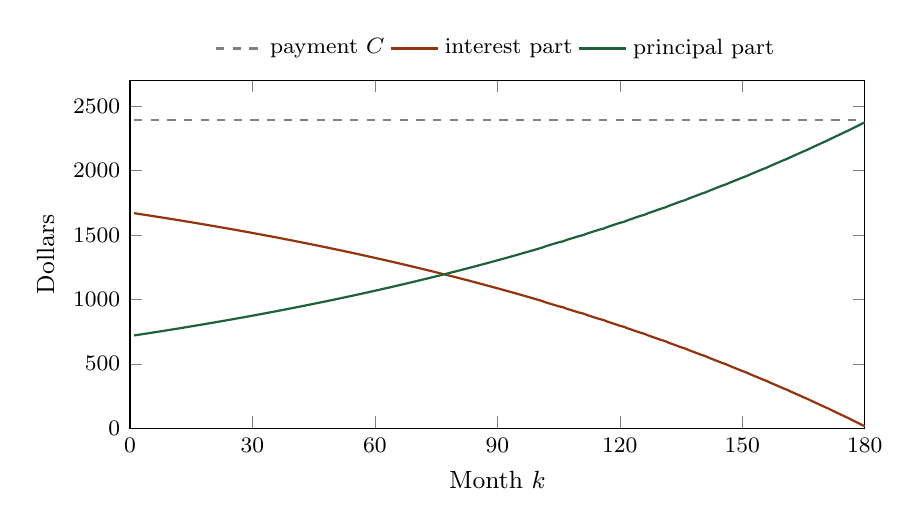
\begin{tikzpicture}
		\begin{axis}[
				width=0.9\textwidth, height=6.0cm,
				xmin=0, xmax=180, ymin=0, ymax=2700,
				xtick={0,30,60,90,120,150,180},
				ytick={0,500,1000,1500,2000,2500},
				xlabel={Month $k$}, ylabel={Dollars},
				label style={font=\small},
				tick label style={font=\footnotesize,
						/pgf/number format/1000 sep={}},
				legend style={font=\footnotesize, at={(0.5,1.03)},
						anchor=south, legend columns=3, draw=none},
				axis line style={thin},
			]
			\addplot[Gray, dashed, thick, domain=1:180, samples=2]
			{2389.1302};
			\addlegendentry{payment $C$}
			\addplot[RawSienna, thick, domain=1:180, samples=180]
			{2389.1302*(1 - (1.0066666667)^(x-181))};
			\addlegendentry{interest part}
			\addplot[SeaGreen!70!black, thick, domain=1:180, samples=180]
			{2389.1302*(1.0066666667)^(x-181)};
			\addlegendentry{principal part}
		\end{axis}
	\end{tikzpicture}
	\caption{Composition of the level monthly payment over the life of the
		loan, computed from the example above. The two parts always sum to $C$,
		and the principal part is a geometric sequence with ratio $1+r/m$.}
	\label{fig:amortization-split}
\end{figure}

\subsection{Calculating the Remaining Principal}

\source{Slides pp.~55--57}

Two ways to answer ``how much is still owed after $k$ payments?''

\subsubsection*{Method 1: run the schedule}

\begin{itemize}[nosep]
	\item A month's principal payment $=$ monthly payment $-$ (previous month's remaining principal) $\times$ (monthly interest rate).
	\item A month's remaining principal $=$ previous month's remaining principal $-$ principal payment calculated above.
	\item Generate the amortization schedule until the particular month you are interested in.
\end{itemize}

This method is relatively slow --- it costs $O(k)$ work --- but it is universal in its applicability.
It can, for example, accommodate prepayments and floating interest rates, neither of which has a closed form.

\subsubsection*{Method 2: discount the remaining cash flows}

Right after the $k$th payment, the remaining principal is the PV of the future $nm-k$ cash flows because we have
\[
    B_{k - 1} (1 + i) - C = B_k
\]
and we can solve this to obtain
\begin{equation}
	B_k = \sum_{i=1}^{nm-k} C\Bigl(1+\frac{r}{m}\Bigr)^{-i}
	= C\,\frac{1-\bigl(1+\frac{r}{m}\bigr)^{-nm+k}}{\frac{r}{m}} .
	\label{eq:remaining}
\end{equation}


This method is much faster --- $O(1)$ instead of $O(k)$ --- but it is limited in applications because it makes more assumptions: a level payment, a fixed rate, and no prepayment.

\begin{exercise}
	Use Eq.~\eqref{eq:remaining} together with Eq.~\eqref{eq:amort-payment} to prove that the \textsf{Principal} column of \autoref{tab:amortization} forms a geometric sequence.
\end{exercise}

\begin{moral}
	The same trade-off as in \autoref{alg:pv-horner}: the closed form is faster, the loop is more general. Which one you may use is decided by the contract, not by the mathematics.
\end{moral}

%─────§ Yields and IRR────────────────────────────────────────────────────────────────────────────────────────────────────────────────────────────
\section{Yields and the Internal Rate of Return}

\source{Slides pp.~58--59}

So far the rate was given and we computed a value.
The rest of the chapter runs the other way: the price is observed in the market, and we solve for the rate it implies.

\subsection{Bond Equivalent Yield and Mortgage Equivalent Yield}

The term \vocab{yield} denotes the return of investment.
Two widely used yields are the \vocab{bond equivalent yield} (BEY) and the \vocab{mortgage equivalent yield} (MEY).
Recall Eq.~\eqref{eq:periodic}, $\mathrm{FV} = \mathrm{PV}\bigl(1+\frac{r}{m}\bigr)^{nm}$:

\begin{itemize}[nosep]
	\item BEY corresponds to the $r$ above that equates PV with FV when $m = 2$.
	\item MEY corresponds to the $r$ above that equates PV with FV when $m = 12$.
\end{itemize}

\begin{observation}
	BEY and MEY may differ numerically, but they refer to the same yield --- they are the same economic fact quoted under two different compounding conventions, exactly as in \autoref{eq:conversion}.
\end{observation}

\begin{remark}
	\vocab{殖利率}（yield）、\vocab{債券等值殖利率}（bond equivalent yield, BEY）、 \vocab{房貸等值殖利率}（mortgage equivalent yield, MEY）。

	上面兩點的意思是：市場給的事實只有「今天付 $\mathrm{PV}$、$n$ 年後拿回 $\mathrm{FV}$」，而年化利率並非事實而是\emph{報價}——必須先選定一年複利幾次，才解得出
	\[
		r = m\left[\left(\frac{\mathrm{FV}}{\mathrm{PV}}\right)^{1/(nm)} - 1\right] ,
	\]
	其值隨 $m$ 而異。
	取 $m = 2$ 者稱 BEY，取 $m = 12$ 者稱 MEY。
	例如今天付 100、一年後拿回 108.16，同一筆現金流可報價為 $8.16\%$（$m = 1$，即\vocab{有效年利率}，effective annual rate）、$8.00\%$（BEY）或 $7.87\%$（MEY）：$m$ 愈大，達成同樣成長所需的\vocab{名目年利率}（nominal rate）愈小。

	兩個名字來自報價慣例——美國公債每半年付息（$m = 2$），房貸每月繳款（$m = 12$）。
	因此跨市場比較前務必先換算，否則會誤判：房貸的 $8\%$ MEY 相當於債券的 $8.13\%$ BEY，兩個 $8\%$ 並不一樣。
\end{remark}

\subsection{The Internal Rate of Return}

\begin{definition}
	The \vocab{internal rate of return} (IRR) is the yield $y$ which equates an investment's PV with its price $P$,
	\[
		P = \frac{C_{1}}{1+y} + \frac{C_{2}}{(1+y)^{2}}
		+ \cdots + \frac{C_{n}}{(1+y)^{n}} .
	\]
\end{definition}

\begin{remark}
	\vocab{內部報酬率}（internal rate of return, IRR）；用在債券上時通常稱 \vocab{到期殖利率}（yield to maturity, YTM）。

	上述定義口語一點的說法是：期初投入 $P$ 元，此後在各個時點分別回收 $C_{1}, \ldots, C_{n}$ 元；\emph{IRR 就是讓這些回收恰好抵掉當初那筆投入的利率}。
	說得再具體些，令 $B_{k}$ 表示第 $k$ 期回收之後\emph{尚未收回}的投資餘額：期初分文未收，故 $B_{0} = P$；此後餘額每期先以利率 $y$ 增值，再扣掉當期收到的 $C_{k}$。
	IRR 就是使餘額在最後一期恰好歸零的那個 $y$：
	\[
		B_{0} = P, \qquad B_{k} = B_{k-1}(1+y) - C_{k}, \qquad B_{n} = 0 .
	\]
	把這條遞迴展開即回到上面的定義式。
	之所以稱為「內部」，是因為算它只用到交易本身的現金流，不必從外部指定折現率。

	\autoref{tab:amortization} 正是這條遞迴的逐期紀錄：餘額每月以 $0.08/12$ 滾息、再減去 2,389.13 元，到第 180 個月剛好歸零。
	所以 $8\%$ 就是那筆房貸對放款人而言的 IRR——我們當初是先給定利率去求月付款，而 IRR 是同一條式子反過來問：給定價格與現金流，利率是多少？

	IRR 的好處是自動把時間價值算進去。
	例如今天付 1,000、往後三年各收回 400，解 $1000 = \sum_{k=1}^{3} 400(1+y)^{-k}$ 得 $y = 9.70\%$；若同樣的 1,200 元要到第三年才一次收到，則只有 $1.2^{1/3}-1 = 6.27\%$。
	總金額相同，但早收到的錢報酬率高得多。

	惟下述再投資假設不可輕忽：承上例，若中途收回的 400 只能以 $3\%$ 再投資，實際年化報酬僅 $7.33\%$，而非宣稱的 $9.70\%$。

	最後，$y$ 在定義式中同時出現在 $n$ 個不同的次方裡，求解 $y$ 等同於解一個 $n$ 次多項式的根，一般沒有公式解，只能用 \autoref{sec:numerical-irr} 的數值方法逼近。
\end{remark}

\begin{remark}
	The IRR assumes all cash flows are reinvested at the \emph{same} rate as the internal rate of return, because
	\[
		\mathrm{FV} = C_{1}(1+y)^{n-1} + C_{2}(1+y)^{n-2} + \cdots + C_{n} .
	\]
	So it must be used with caution.
	The issue disappears when there are no intermediate cash flows --- which is one reason zero-coupon bonds (\autoref{sec:zero-coupon}) are so convenient.
\end{remark}

%─────§ Numerical methods──────────────────────────────────────────────────────────────────────────────────────────────────────────────────────────
\section{Numerical Methods for IRRs}
\label{sec:numerical-irr}

\source{Slides pp.~60--69}

\subsection{The Root-Finding Problem}

Define
\[
	f(y) \;\triangleq\; \sum_{t=1}^{n} \frac{C_{t}}{(1+y)^{t}} - P ,
\]
where $P$ is the market price, and solve $f(y) = 0$ for a real $y \ge -1$.\footnote{Negative interest rates became a reality for German and Swiss bonds in 2015.
In 2016, Sweden, Denmark, and Japan imposed negative interest rates on excess reserves.
As many as 355 corporate bonds were issued with negative yields as of June of 2016.
Even so, $-100\%$ should be a natural lower bound because why would anyone or financial institutions want to have every cent confiscated?}

\begin{proposition}
	If $C_{t} > 0$ for all $t$, then $f(y)$ is monotonically decreasing in $y$, so a unique real-number solution exists.
	\label{prop:irr-unique}
\end{proposition}

There is no closed form for $y$ in general, so we need iterative methods.
The three below trade off robustness against speed.

\begin{remark}
	\emph{Trade off A against B} 意為在 A 與 B 之間權衡取捨：想多要一點 B，就得犧牲一些 A。
	此處的兩個軸是\vocab{穩健性}（robustness，是否保證收斂、對起始值是否敏感）與\vocab{速度}（收斂階數），三者的對照見 \autoref{tab:rootfinding}。

	二分法最穩健：只要初始區間滿足 $f(a)f(b) < 0$ 便保證收斂，但每步僅將區間減半，故最慢。
	牛頓法與割線法則\emph{都不保證收斂}。
	例如 $f(x) = x^{1/3}$ 的牛頓疊代為 $x_{k+1} = x_{k} - 3x_{k} = -2x_{k}$，自任何非零起點出發都翻倍發散；而 $f(x) = x^{3}-2x+2$ 自 $x_{0} = 0$ 出發則在 $0 \leftrightarrow 1$ 之間永遠循環，一步都不前進。
	此外 $f'(x_{k}) \approx 0$ 時步長會爆炸，多根時亦可能收斂到非預期的那一個；割線法還多一個分母 $f(x_{k})-f(x_{k-1})$ 趨零的風險。
	理論上能保證的只有\emph{局部}收斂：起點充分接近單根時保證二次收斂，但定理並未告訴你「充分接近」究竟是多近。

	不過就 IRR 這個問題而言，\autoref{prop:irr-unique} 其實已把風險排除了。
	當所有 $C_{t} > 0$ 時 $f$ 不僅單調遞減，還滿足 $f''(y) = \sum_{t} t(t+1)C_{t}(1+y)^{-t-2} > 0$ 而為凸函數。
	凸函數的切線恆在曲線下方，故 $f(x_{k+1}) \geq 0$；又 $f$ 遞減，這表示第一步之後每個迭代點都落在根的左側。
	此後 $f(x_{k}) \geq 0$ 而 $f'(x_{k}) < 0$，步長 $-f/f'$ 恆非負，迭代遂單調遞增且以根為上界，必定收斂。
	所以該命題不只是在說「根唯一」，更是在替牛頓法背書：對付息全為正的 IRR，牛頓法自任何 $y_{0} > -1$ 出發都保證收斂。

	實務上的求根程式（如 Brent's method）多半混用：先以二分法將根框住，再切換至割線或牛頓法加速，一旦迭代點跳出括號便退回二分法——保證來自二分法，速度來自另外兩者。
\end{remark}

\subsection{The Bisection Method}

Start with $a$ and $b$ where $a < b$ and $f(a)\,f(b) < 0$.
Then $f(\xi)$ must be zero for some $\xi \in [\,a,b\,]$.
If we evaluate $f$ at the midpoint $c \triangleq (a+b)/2$, either

\begin{enumerate}[nosep, label=(\arabic*)]
	\item $f(c) = 0$,
	\item $f(a)\,f(c) < 0$, or
	\item $f(c)\,f(b) < 0$.
\end{enumerate}

In the first case we are done; in the second we continue the process with the new bracket $[\,a,c\,]$; and in the third we continue with $[\,c,b\,]$.
The bracket is halved in the latter two cases, so after $n$ steps $\xi$ lies within a bracket of length $(b-a)/2^{n}$.

\begin{figure}[H]
	\centering
	\begin{tikzpicture}[font=\small]
		\draw[-{Stealth[length=5pt]}] (0,-1.7) -- (0,2.7);
		\draw[-{Stealth[length=5pt]}] (-0.35,0) -- (7.3,0);
		\draw[MidnightBlue!75!black, thick, domain=0.35:6.7, samples=100,
			smooth, variable=\x]
		plot ({\x}, {3.2/(\x+0.55) - 0.75});
		\foreach \x/\lbl in {2.4/a, 3.6/c, 4.8/b} {
				\draw (\x,0.13) -- (\x,-0.13);
				\node[below=1pt] at (\x,-0.13) {$\lbl$};
			}
	\end{tikzpicture}
	\caption{The bisection method. $f$ is decreasing with $f(a)>0>f(b)$, so the
		root is bracketed; evaluating at $c$ halves the bracket.}
	\label{fig:bisection}
\end{figure}

\subsection{The Newton--Raphson Method}

It converges faster than the bisection method.
Start with a first approximation $x_{0}$ to a root of $f(x) = 0$.
Then
\[
	x_{k+1} \;\triangleq\; x_{k} - \frac{f(x_{k})}{f'(x_{k})} .
\]
When computing yields,
\begin{equation}
	f'(x) = -\sum_{t=1}^{n} \frac{t\,C_{t}}{(1+x)^{t+1}} .
	\label{eq:newton-deriv}
\end{equation}

\begin{figure}[H]
	\centering
	\begin{tikzpicture}[font=\small]
		\draw[-{Stealth[length=5pt]}] (0,-2.4) -- (0,1.6) node[left] {$y$};
		\draw[-{Stealth[length=5pt]}] (-0.35,0) -- (9.5,0) node[right] {$x$};
		\draw[MidnightBlue!75!black, thick, domain=0:9, samples=100,
			smooth, variable=\x]
		plot ({\x}, {1.8*(2.0 - 7/(0.35*\x + 2.2))});
		% x_k = 1, f(x_k) = -1.3412; x_{k+1} = 2.978
		\draw[dashed, Gray] (1,0) -- (1,-1.3412);
		\draw[dashed, RawSienna, thick] (0.6,-1.6124) -- (3.6,0.4193);
		\node[above=3pt] at (1,0) {$x_{k}$};
		\node[above=5pt] at (2.978,0) {$x_{k+1}$};
		\node[right] at (9,1.05) {$f(x)$};
	\end{tikzpicture}
	\caption{The Newton--Raphson method. The tangent at $x_{k}$ is followed to
		the axis to give $x_{k+1}$.}
	\label{fig:newton}
\end{figure}

\subsection{The Secant Method}

A variant of the Newton--Raphson method: replace differentiation with difference.
Start with two approximations $x_{0}$ and $x_{1}$, then compute the $(k+1)$st approximation with
\[
	x_{k+1} = x_{k} - \frac{f(x_{k})\,(x_{k}-x_{k-1})}{f(x_{k})-f(x_{k-1})} ,
\]
so $[\,f(x_{k})-f(x_{k-1})\,]/(x_{k}-x_{k-1})$ replaces $f'(x_{k})$.

\begin{figure}[H]
	\centering
	\begin{tikzpicture}[font=\small]
		\draw[-{Stealth[length=5pt]}] (0,-2.4) -- (0,1.6) node[left] {$y$};
		\draw[-{Stealth[length=5pt]}] (-0.35,0) -- (9.5,0) node[right] {$x$};
		\draw[MidnightBlue!75!black, thick, domain=0:9, samples=100,
			smooth, variable=\x]
		plot ({\x}, {1.8*(2.0 - 7/(0.35*\x + 2.2))});
		% x_{k-1} = 1, f = -1.3412; x_k = 7, f = 0.8903; the chord meets the axis at 4.606
		\draw[dashed, Gray] (1,0) -- (1,-1.3412);
		\draw[dashed, Gray] (7,0) -- (7,0.8903);
		\draw[RawSienna, thick] (0.4,-1.5644) -- (8.2,1.3366);
		\fill[MidnightBlue!75!black] (1,-1.3412) circle (1.6pt);
		\fill[MidnightBlue!75!black] (7,0.8903) circle (1.6pt);
		\node[above=3pt] at (1,0) {$x_{k-1}$};
		\node[below=3pt] at (7,0) {$x_{k}$};
		\node[below=3pt] at (4.606,0) {$x_{k+1}$};
		\node[right] at (9,1.05) {$f(x)$};
	\end{tikzpicture}
	\caption{The secant method. The chord through the two latest iterates is
		followed to the axis to give $x_{k+1}$; compare \autoref{fig:newton},
		which follows the tangent at a single iterate instead.}
	\label{fig:secant}
\end{figure}

Its convergence rate is $1.618$, slightly worse than the Newton--Raphson method's $2$.
But the secant method does not evaluate $f'(x_{k})$, which saves about $50\%$ in computation efforts per iteration.
For reference, the convergence rate of the bisection method is $1$.

\begin{table}[H]
	\centering
	\begin{tabular}{@{}l c c l@{}}
		\toprule
		Method           & Convergence rate & Needs $f'$? & Convergence guaranteed?      \\
		\midrule
		Bisection        & $1$              & no          & yes, once bracketed          \\
		Secant           & $1.618$          & no          & no                           \\
		Newton--Raphson  & $2$              & yes         & no (see \autoref{prop:irr-unique}) \\
		\bottomrule
	\end{tabular}
	\caption{The three root-finding methods. Higher rate means fewer iterations,
		but each Newton--Raphson iteration costs roughly twice a secant one --- and
		the last column is what that speed is bought with. Bisection cannot fail
		once $f(a)f(b) < 0$; the other two may diverge, cycle, or land on the wrong
		root.}
	\label{tab:rootfinding}
\end{table}

\begin{remark}
	\vocab{割線法}（secant method）的幾何意義見 \autoref{fig:secant}：牛頓法在\emph{一個}點上作切線、追到 $x$ 軸得下一個近似值，割線法則改取\emph{最近兩個}點連成的割線，追到 $x$ 軸得下一個近似值——名稱即由此而來。
	公式也是這樣來的：通過 $(x_{k-1}, f(x_{k-1}))$ 與 $(x_{k}, f(x_{k}))$ 的直線斜率為差商 $[f(x_{k})-f(x_{k-1})]/(x_{k}-x_{k-1})$，令該直線的 $y$ 座標為零解出交點，就得到上式。
	換言之，割線法就是把牛頓法裡的 $f'(x_{k})$ 換成差商——用兩點的\emph{實際落差}去估斜率，而不去要求函數可微或另外寫一份導數程式。

	所謂省下約 $50\%$ 的計算量，關鍵在於 $f(x_{k-1})$ 在上一輪就已經算過、可直接沿用，故每輪只需\emph{一次}新的函數求值；牛頓法每輪則要各算一次 $f$ 與 $f'$，而由 \eqref{eq:newton-deriv} 可見算 $f'$ 的成本與算 $f$ 相當。
	若改以每次函數求值（而非每輪疊代）來衡量效率，牛頓法為 $2^{1/2} \approx 1.414$、割線法為 $1.618$：\emph{割線法反而略勝一籌}。

	至於 $1.618$ 這個怪數字，來自誤差遞迴 $e_{k+1} \approx C\,e_{k}e_{k-1}$：設 $e_{k+1} \sim A\,e_{k}^{p}$ 代入可得 $p^{2} = p+1$，故 $p = (1+\sqrt{5})/2$，恰為黃金比例。

	最後可與二分法對照：兩者都持有兩個點，但二分法只看 $f$ 的\emph{正負號}並取中點，割線法則利用 $f$ 的\emph{數值大小}外推。
	多用了資訊所以更快，代價是失去保證——割線法不保證收斂，且當 $f(x_{k}) \approx f(x_{k-1})$ 時分母趨近於零，數值上會不穩定。
\end{remark}

\subsection{Systems of Nonlinear Equations}

It is not easy to extend the bisection method to higher dimensions --- there is no natural notion of ``bracketing'' a root in the plane.
But the Newton--Raphson method extends directly.

Let $(x_{k}, y_{k})$ be the $k$th approximation to the solution of the two simultaneous equations
\[
	f(x,y) = 0, \qquad g(x,y) = 0 .
\]
The $(k+1)$st approximation $(x_{k+1}, y_{k+1})$ satisfies the following \emph{linear} equations,
\[
	\begin{bmatrix}
		\dfrac{\partial f(x_{k},y_{k})}{\partial x} &
		\dfrac{\partial f(x_{k},y_{k})}{\partial y}   \\[2ex]
		\dfrac{\partial g(x_{k},y_{k})}{\partial x} &
		\dfrac{\partial g(x_{k},y_{k})}{\partial y}
	\end{bmatrix}
	\begin{bmatrix}
		\Delta x_{k+1} \\[2ex] \Delta y_{k+1}
	\end{bmatrix}
	= -
	\begin{bmatrix}
		f(x_{k},y_{k}) \\[2ex] g(x_{k},y_{k})
	\end{bmatrix} ,
\]
with unknowns
\[
	\Delta x_{k+1} \triangleq x_{k+1}-x_{k},
	\qquad
	\Delta y_{k+1} \triangleq y_{k+1}-y_{k} .
\]
The above has a unique solution for $(\Delta x_{k+1}, \Delta y_{k+1})$ when the $2\times 2$ matrix --- the Jacobian --- is invertible.
Finally, set
\[
	x_{k+1} = x_{k} + \Delta x_{k+1},
	\qquad
	y_{k+1} = y_{k} + \Delta y_{k+1} .
\]

\begin{intuition}
	Each step replaces the nonlinear system by its linearisation at the current point and solves that exactly.
	In one dimension the linearisation is the tangent line of \autoref{fig:newton}; here it is the tangent plane.
\end{intuition}

\begin{remark}
	這節處理的是「$n$ 條方程式、$n$ 個未知數，且方程式非線性」的情形，前面求 IRR 不過是 $n = 1$ 的特例。
	金融上最常見的來源是\vocab{校準}（calibration）：以市場上觀測到的 $n$ 個價格，反解出模型的 $n$ 個未知參數——例如用兩檔債券的市價反推某個兩參數利率模型的兩個參數。

	二分法之所以推不到高維，是因為它的保證來自中間值定理：一維上 $f$ 一變號就把根夾住了。
	但在平面上 $f(x,y) = 0$ 的解集通常是一條\emph{曲線}而非一個點，我們要的是它與 $g(x,y) = 0$ 那條曲線的\emph{交點}；此時並沒有「把區域對半切、且能判斷根落在哪一半」的辦法，\vocab{框住根}（bracketing）這個概念本身就不存在。

	至於那條矩陣方程式並非憑空而來，它就是一階泰勒展開後令其為零。
	在 $(x_{k}, y_{k})$ 附近，
	\[
		f(x_{k+1}, y_{k+1}) \approx f(x_{k},y_{k})
		+ \frac{\partial f}{\partial x}\,\Delta x_{k+1}
		+ \frac{\partial f}{\partial y}\,\Delta y_{k+1} ,
	\]
	$g$ 亦然。
	我們\emph{希望}新的一點恰好是解，於是令兩式右側皆為零、把常數項移到等號另一邊，寫成矩陣形式就是上式。

	因此這整套做法與一維的牛頓法其實是同一件事。
	把該矩陣方程記為 $J\Delta = -F$，則 $\Delta = -J^{-1}F$，亦即 $\mathbf{x}_{k+1} = \mathbf{x}_{k} - J^{-1}F(\mathbf{x}_{k})$：一維的「除以導數 $f'(x_{k})$」在多維成了「左乘 Jacobian 的反矩陣」，而一維要求 $f'(x_{k}) \neq 0$ 也正對應到此處要求 $J$ 可逆。
	繞這一圈的用意則在於，非線性方程組難解，線性方程組卻可直接以高斯消去法解出。
\end{remark}

%─────§ Bonds─────────────────────────────────────────────────────────────────────────────────────────────────────────────────────────────────────
\section{Bonds}

\source{Slides pp.~70--74}

\subsection{Zero-Coupon Bonds}
\label{sec:zero-coupon}

\begin{definition}
	A \vocab{zero-coupon bond} (or \vocab{pure discount bond}) makes a single payment at maturity.
	By Eq.~\eqref{eq:fv-pv}, the price of one that pays $F$ dollars in $n$ periods is
	\begin{equation}
		F/(1+r)^{n} , \label{eq:zero-price}
	\end{equation}
	where $r$ is the interest rate per period.
\end{definition}

Zero-coupon bonds can be used to meet future obligations as there is no reinvestment risk --- the caveat attached to the IRR above simply does not arise.

\begin{remark}
	\vocab{零息債券}（zero-coupon bond），亦稱\vocab{純折價債券}（pure discount bond）；$F$ 為\vocab{面值}（par value，即票面金額），$n$ 為到期期數。
	口語地說，它就是一張「中途完全不付息、到期一次付你一筆固定金額」的債券——正因為中途沒有任何\vocab{票息}（coupon），才叫「零息」。
	它的報酬全部來自\emph{買價與面值之間的價差}：由 \eqref{eq:zero-price} 可知，只要 $r > 0$ 價格便必然低於面值，即必定\emph{折價}發行，故又稱純折價債券。

	上段所謂沒有\vocab{再投資風險}（reinvestment risk），指的正是先前 IRR 那條但書在此不成立：中途沒有現金流，就沒有錢需要再投資，也就無從假設再投資利率。
	因此零息債券的 IRR 就是你實際拿到的報酬，一分不差；這也是為何它適合用來支應未來某個時點的確定支出。

	例中 $20.83$ 這個數字採債券市場的報價慣例——以\emph{面額 100} 為基準，故 $20.83$ 意為面額 100 元的債券今天只賣 $20.83$ 元。
	另可留意 $45.64\% \times 45.64\% \approx 20.83\%$：20 年期的價格恰為 10 年期價格的平方，因為折現是連乘而非相加。
\end{remark}

\begin{eg}
	The interest rate is $8\%$ compounded semiannually.
	A zero-coupon bond that pays the par value 20 years from now will be priced at $1/(1.04)^{40}$, that is, $20.83\%$ of its par value.\footnote{One fifth!} It will be quoted as $20.83$.
	If the bond matures in 10 years instead of 20, its price would be $45.64$.
\end{eg}

\subsection{Level-Coupon Bonds}

A \vocab{level-coupon bond} is described by its \vocab{coupon rate} and its \vocab{par value}, paid at maturity.
Write $F$ for the par value and $C$ for the coupon.

\begin{remark}
	\label{rmk:level-coupon}
	\vocab{固定票息債券}（level-coupon bond，亦稱附息債券）；$c$ 為\vocab{票面利率}（coupon rate），$F$ 為\vocab{面值}（par value），$C$ 為每期的\vocab{票息}（coupon）。
	口語地說，它就是「每期付你固定的 $C$ 元，到期那一期除了 $C$ 之外再一次還你 $F$ 元」的債券，現金流見 \autoref{fig:coupon-cashflow}。
	留意原文的 \emph{paid at maturity} 修飾的是 par value 而非 coupon rate：票息是\emph{每期}都付，面值則是\emph{到期}才一次付清。
	所謂 \emph{level}（等額）是指每期票息固定不變，以與浮動利率債券相區別。

	票面利率與票息的換算為下文的 $C = Fc/m$：$c$ 是\emph{年}利率，乘上面值得一年的總票息，再除以一年付息次數 $m$ 即為每期票息。
	例如面值 100、票面利率 $8\%$、每半年付息一次，則 $m = 2$、每期票息 $C = 100 \times 0.08/2 = 4$ 元。

	最要緊的是分清 $c$ 與 $r$ 這兩個利率：$c$ 由合約寫死，決定你每期\emph{收到多少錢}，發行後永不改變；$r$ 則是市場折現率，隨市場浮動，決定這串現金流\emph{今天值多少錢}。
	兩者的大小關係恰好決定債券售價高於、等於或低於面值，即\vocab{溢價}（premium）、\vocab{平價}（par）與\vocab{折價}（discount）三種情形：當 $c = r$ 時 $C = Fr/m$，代入 \eqref{eq:bond-price} 後前項化為 $F\bigl[1-(1+\frac{r}{m})^{-n}\bigr]$，與後項 $F(1+\frac{r}{m})^{-n}$ 相加恰得 $P = F$；又 $P$ 對 $r$ 遞減，故
	\[
		c = r \implies P = F\ (\text{平價}), \qquad
		c < r \implies P < F\ (\text{折價}), \qquad
		c > r \implies P > F\ (\text{溢價}) .
	\]
	而 $c = 0$ 即退化為前一小節的零息債券，價格恰為 \eqref{eq:zero-price}——零息債券只是本式的特例。
\end{remark}

\begin{figure}[H]
	\centering
	\begin{tikzpicture}[font=\small]
		\draw[-{Stealth[length=6pt]}] (-0.3,0) -- (9.6,0);
		\foreach \x/\lbl in {1.7/1, 3.4/2, 5.1/3} {
				\draw[-{Stealth[length=5pt]}, thick] (\x,0) -- (\x,0.75);
				\node[above=1pt] at (\x,0.75) {$C$};
				\node[below=2pt] at (\x,0) {$\lbl$};
			}
		\node at (6.3,0.5) {$\cdots$};
		\draw[-{Stealth[length=5pt]}, very thick] (7.5,0) -- (7.5,1.35);
		\node[above=1pt] at (7.5,1.35) {$C+F$};
		\node[below=2pt] at (7.5,0) {$n$};
	\end{tikzpicture}
	\caption{The cash flow of a level-coupon bond.}
	\label{fig:coupon-cashflow}
\end{figure}

\begin{remark}
	\autoref{fig:coupon-cashflow} 隱含一項理想化的假設：\emph{今天恰好站在付息日上}，故各筆現金流剛好落在 $1, 2, \ldots, n$ 這些整數期上。
	真實的交割日多半落在兩個付息日之間，屆時每一筆現金流都要往前挪，指數由 $i$ 變成 $\omega + i$——這正是 \eqref{eq:full-price} 所處理的情形。

	不過要留意，\emph{最後一期同時收到 $C$ 與 $F$ 並非理想化}，真實債券的最後一次付息本就與本金同日支付。
	這一點在 \eqref{eq:full-price} 中依然成立：末筆票息（$i = n-1$）與 $F$ 的折現指數同為 $\omega+n-1$，可見放寬假設後兩者仍同時發生。
\end{remark}

\begin{moral}
	Coupon bonds can be thought of as a matching package of zero-coupon bonds, at least theoretically.\footnote{``You see, Daddy didn't bake the cake, and Daddy isn't the one who gets to eat it.
	But he gets to slice the cake and hand it out.
	And when he does, little golden crumbs fall off the cake.
	And Daddy gets to eat those,'' wrote Tom Wolfe (1931--2018) in \emph{Bonfire of the Vanities} (1987).}
\end{moral}

\begin{remark}
	這條 moral 的具體意思是：一張 $n$ 期的附息債券，可視為 $n$ 張面額 $C$、到期日分別為 $1, 2, \ldots, n$ 的零息債券，再加上一張面額 $F$、到期日為 $n$ 的零息債券，所組成的投資組合。
	下方的定價公式 \eqref{eq:bond-price} 正是把這個拆解逐項寫出來：第一項是 $n$ 張票息零息債券的現值之和，第二項則是面值那一張的現值。

	所謂 \emph{at least theoretically}，是指這種拆解未必真能在市場上執行；但在美國公債市場它確實可行。
	自 1985 年起的 \vocab{STRIPS} 制度（Separate Trading of Registered Interest and Principal of Securities）允許交易商將一張公債的每一期票息與本金拆開、各自登記為獨立的零息債券單獨買賣，亦允許反向\emph{重組}回原債券。
	雙向皆可執行，套利便會迫使「整張債券的價格」等於「各零息碎片價格之和」——這條 moral 因而不只是心算技巧，而是由無套利條件所保證。

	這個觀點日後還有一個更要緊的用處：拆開之後每一張零息債券各有自己的到期日，理應各用\emph{該期限的即期利率}折現。
	\eqref{eq:bond-price} 對所有期別一律套用單一的 $r$，其實是一種簡化，正確的做法是改用一整條利率期限結構。

	至於註腳的典故，出自 Tom Wolfe 的小說 \emph{Bonfire of the Vanities}（1987）：書中債券業務員 Sherman McCoy 的妻子向女兒解釋爸爸的工作——蛋糕不是爸爸烤的，也不是爸爸吃的，但由爸爸負責切開、分送給大家；切的時候會掉下金色的碎屑，那些碎屑就歸爸爸。
	放在此處是一語雙關：交易商正是把債券「切片」（strip）後分銷，自己既不創造現金流也不領取現金流，賺的就是買賣價差那些「碎屑」。
\end{remark}

Splitting the cash flow of \autoref{fig:coupon-cashflow} into an annuity of coupons plus a zero-coupon bond for the par value, and applying Eq.~\eqref{eq:gen-annuity} and Eq.~\eqref{eq:zero-price}, gives the pricing formula
\begin{align}
	P & = \sum_{i=1}^{n} \frac{C}{\bigl(1+\frac{r}{m}\bigr)^{i}}
	+ \frac{F}{\bigl(1+\frac{r}{m}\bigr)^{n}} \nonumber                          \\
	  & = C\,\frac{1-\bigl(1+\frac{r}{m}\bigr)^{-n}}{\frac{r}{m}}
	+ \frac{F}{\bigl(1+\frac{r}{m}\bigr)^{n}} . \label{eq:bond-price}
\end{align}
Here $n$ is the number of cash flows, $m$ the number of payments per year, and $r$ the annual rate compounded $m$ times per annum.
Note $C = Fc/m$ when $c$ is the annual coupon rate.


\begin{note}
	Because the sum collapses to a closed form, the price $P$ can be computed in $O(1)$ time --- no loop over the $n$ coupons is needed.
\end{note}

\subsection{Yields to Maturity}

\begin{definition}
	The \vocab{yield to maturity} (YTM) is the $r$ that satisfies Eq.~\eqref{eq:bond-price} with $P$ being the bond price.
\end{definition}

\begin{eg}
	For a $15\%$ BEY, a 10-year bond with a coupon rate of $10\%$ paid semiannually sells for
	\[
		5 \times \frac{1-[\,1+(0.15/2)\,]^{-2\times 10}}{0.15/2}
		+ \frac{100}{[\,1+(0.15/2)\,]^{2\times 10}}
		= 74.5138
	\]
	percent of par.
	So $15\%$ is the yield to maturity if the bond sells for $74.5138$.\footnote{Note that the yield $15\%$ exceeds the coupon rate $10\%$.}
\end{eg}

\begin{remark}
	\vocab{到期殖利率}（yield to maturity, YTM）的名稱可拆成兩半來理解：\emph{yield} 指報酬率，\emph{to maturity} 則指這個報酬率是在「\emph{一路持有到到期日}」的前提下算出來的。
	換言之它回答的是：若今天以價格 $P$ 買進、此後每期領取票息、到期領回面值且中途不賣出，這串現金流相當於年利率多少？

	之所以要把持有期間寫進名字裡，是因為債券還有別的「殖利率」，各自假設不同的持有期間。
	\vocab{當期收益率}（current yield）$= Cm/P$ 只比較票息收入與價格，完全不管到期時的資本利得或損失——以上例而言其值為 $10/74.5138 = 13.42\%$，低於 YTM 的 $15\%$，差額正是價格將由 $74.51$ 回升至面值 $100$ 的那段資本利得。
	\vocab{贖回殖利率}（yield to call）則假設持有至發行人提前贖回之日而非到期日；若中途賣出，實際得到的又是另一個持有期報酬率。
	既然數字取決於你假設持有多久，名字裡自然得講明是哪一種。

	至於它與前面 IRR 的關係：YTM 就是把 \eqref{eq:bond-price} 反解 $r$，亦即債券這筆投資的 IRR，只是債券市場習慣改稱 YTM。
	因此 IRR 的但書一併繼承：YTM 要成為你\emph{實際}拿到的報酬，除了持有到期、發行人不違約之外，還須能把每一期收到的票息都以 $r$ 再投資出去。
	零息債券沒有中途票息、無從再投資，其 YTM 恰為實際報酬——這正是前面說它「沒有再投資風險」的意思。

	儘管有這些但書，YTM 仍是債券市場的標準報價，因為它把價格、票息與到期日壓縮成單一數字，使票面利率與年期各異的債券得以直接比較。
\end{remark}

\subsection{Price Behavior}

\source{Slides pp.~75--79}

\subsubsection*{(1) Direction}

Bond prices fall when interest rates rise, and vice versa.
This is immediate from Eq.~\eqref{eq:bond-price} --- every term is decreasing in $r$ --- and yet ``only 24 percent answered the question correctly.''\footnote{CNN, December 21, 2001.}

\begin{remark}
	價格與市場利率反向的道理在於：票息 $C$ 與面值 $F$ 已由合約寫死，市場利率變動改變的\emph{不是你會收到多少錢，而是那些錢今天值多少}。
	利率上升時，新發行的債券給得更多，你手上這張給得少的自然得降價才賣得掉；利率下跌則反之。
	註腳所引 2001 年 CNN 的調查中僅 $24\%$ 的人答對，正是因為多數人誤把「利率上升」聯想成「債券更值錢」——真正在變動的是折現率，而非票息。
\end{remark}

\subsubsection*{(2) Premium, par, and discount}

A level-coupon bond sells\footnote{Consult the text for proofs.}

\begin{itemize}[nosep]
	\item at a \vocab{premium} (above its par value) when its coupon rate $c$ is above the market interest rate $r$;
	\item at \vocab{par} (at its par value) when its coupon rate is equal to the market interest rate;
	\item at a \vocab{discount} (below its par value) when its coupon rate is below the market interest rate.
\end{itemize}

Bonds selling at par, at a premium and at a discount are called \vocab{par bonds}, \vocab{premium bonds} and \vocab{discount bonds} respectively.

\begin{table}[H]
	\centering
	\begin{tabular}{@{}c c@{}}
		\toprule
		Yield (\%) & \begin{tabular}[b]{@{}c@{}}Price\\(\% of par)\end{tabular} \\
		\midrule
		7.5              & 113.37                                              \\
		8.0              & 108.65                                              \\
		8.5              & 104.19                                              \\
		\textbf{9.0}     & \textbf{100.00}                                     \\
		9.5              & 96.04                                               \\
		10.0             & 92.31                                               \\
		10.5             & 88.79                                               \\
		\bottomrule
	\end{tabular}
	\caption{A $9\%$ coupon bond. The bond trades at par exactly when the yield
		equals the coupon rate (bold row), at a premium above, at a discount below.}
	\label{tab:coupon9}
\end{table}

\begin{remark}
	\vocab{溢價}（premium）、\vocab{平價}（par）與\vocab{折價}（discount）；依售價分類者分別稱為\vocab{平價債券}（par bonds）、\vocab{溢價債券}（premium bonds）與\vocab{折價債券}（discount bonds）。
	三者的定義與判準已見 \autoref{rmk:level-coupon}：$c = r$ 時 $P = F$，且 $P$ 對 $r$ 遞減，故 $c > r$ 時售價高於面值（溢價）、$c < r$ 時低於面值（折價）。

	以下補上溢價與折價的金額。
	記 $a \triangleq \bigl[1-(1+\frac{r}{m})^{-n}\bigr]\big/\frac{r}{m}$ 為年金現值因子，則代入 $C = Fc/m$ 後，\eqref{eq:bond-price} 可寫成 $P = \frac{Fc}{m}\,a + F(1+\frac{r}{m})^{-n}$。
	在同一式中把 $c$ 換成 $r$，右側恰化簡為 $F$，於是有恆等式 $F = \frac{Fr}{m}\,a + F(1+\frac{r}{m})^{-n}$——這正是平價的情形。
	兩式相減，末項相消，故
	\[
		P - F = \frac{F(c-r)}{m}\,a
		= \sum_{i=1}^{n} \frac{\;\dfrac{F(c-r)}{m}\;}
		{\bigl(1+\frac{r}{m}\bigr)^{i}} ,
	\]
	末式是把 $a = \sum_{i=1}^{n}(1+\frac{r}{m})^{-i}$ 展開的結果，意思一目了然：\emph{第 $i$ 期你比市場行情多領（或少領）$F(c-r)/m$ 元，把這 $n$ 筆差額各自折現回今天再加總，就是溢價（或折價）的金額}。

	以 \autoref{tab:coupon9} 的 $9\%$ 債券驗證：殖利率 $8\%$ 時每期多領 $0.5$ 元，$a = 17.292$，故 $P - F = 0.5 \times 17.292 = 8.65$，恰為表中 $108.65$ 與面值 $100$ 之差。
	另可留意，無論溢價或折價，到期時價格必然回到面值，故溢價債券的價格會隨時間逐步下滑至 $F$——那是溢價的攤銷，並非虧損。
\end{remark}

\begin{remark}
	在此說明如何讀 \autoref{tab:coupon9}。
	表中描述的是一張 15 年期、票面利率 $c = 9\%$、每半年付息一次的債券，即 $n = 30$、$m = 2$、每期票息 $C = Fc/m = 4.5$ 元；\emph{整張表自始至終都是這同一張債券}，票面利率固定為 $9\%$ 不變。
	變動的只有左欄的市場殖利率 $r$，右欄則是把該 $r$ 代入 \eqref{eq:bond-price} 算得的價格，並依債券市場慣例以面額 100 為基準表示（故 $100.00$ 即等於面值）。
	例如第一列 $r = 7.5\%$：$a = \bigl[1-(1.0375)^{-30}\bigr]\big/0.0375 = 17.829$，$P = 4.5 \times 17.829 + 100 \times (1.0375)^{-30} = 113.37$，與表中相符。
	粗體列即 $r = c = 9\%$ 的平價情形；其\emph{上方}各列殖利率較低故溢價，\emph{下方}各列殖利率較高故折價——留意表格說明裡的 \emph{above}／\emph{below} 指的是粗體列的上下方，而非殖利率的高低。
	這七列也就是 \autoref{fig:convexity} 曲線上標出的七個點。
\end{remark}

\subsubsection*{(3) Convexity}

The price--yield relationship is not merely decreasing; it is \emph{convex}.
Concretely, take any yield change of size $\Delta > 0$.
The price \emph{gain} from a fall of $\Delta$ is larger than the price \emph{loss} from a rise of that same $\Delta$,
\[
	P(r-\Delta) - P(r) \;>\; P(r) - P(r+\Delta) ,
\]
and the gap widens as $\Delta$ grows.

\begin{figure}[H]
	\centering
	\begin{tikzpicture}
		\begin{axis}[
				width=0.9\textwidth, height=6.2cm,
				xmin=0, xmax=0.21, ymin=0, ymax=220,
				xtick={0,0.05,0.10,0.15,0.20},
				ytick={0,50,100,150,200},
				xlabel={Yield}, ylabel={Price (\% of par)},
				label style={font=\small},
				tick label style={font=\footnotesize,
						/pgf/number format/fixed,
						/pgf/number format/precision=3},
				axis line style={thin},
				legend style={font=\footnotesize, at={(0.97,0.95)},
						anchor=north east, draw=none},
			]
			\addplot[MidnightBlue!75!black, thick, domain=0.01:0.21, samples=120]
			{4.5*(1-(1+x/2)^(-30))/(x/2) + 100*(1+x/2)^(-30)};
			\addlegendentry{price--yield curve}
			\addplot[only marks, mark=*, mark size=1.3pt, RawSienna] coordinates {
					(0.075,113.37) (0.080,108.65) (0.085,104.19) (0.090,100.00)
					(0.095,96.04) (0.100,92.31) (0.105,88.79)
				};
			\addlegendentry{rows of \autoref{tab:coupon9}}
		\end{axis}
	\end{tikzpicture}
	\caption{Convexity of the price--yield curve, for the 15-year, $9\%$ coupon
		bond paid semiannually that generates \autoref{tab:coupon9}. The seven
		tabulated prices are marked; they lie on the curve.}
	\label{fig:convexity}
\end{figure}

\begin{remark}
	凸性即 $\partial^{2}P/\partial r^{2} > 0$：\eqref{eq:bond-price} 的每一項皆形如 $A\bigl(1+\frac{r}{m}\bigr)^{-i}$，其二階導數 $\frac{i(i+1)A}{m^{2}}\bigl(1+\frac{r}{m}\bigr)^{-i-2} > 0$，逐項為凸，總和自然為凸。
	其實際意涵是漲跌不對稱：由 \autoref{tab:coupon9}，殖利率自 $9\%$ 降至 $8\%$ 價格漲 $8.65$，升至 $10\%$ 卻只跌 $7.69$，且幅度愈大這個不對稱愈明顯。
	換言之利率無論往哪個方向變動同樣幅度，持有人\emph{賺的總是多於賠的}，故凸性本身即具價值，市場會為凸性較高的債券付出較高的價格——這是日後存續期間與凸性避險的基礎。
\end{remark}


%─────§ Day count conventions─────────────────────────────────────────────────────────────────────────────────────────────────────────────────────
\section{Day Count Conventions}

\source{Slides pp.~80--83}

Every formula above assumed cash flows land on exact period boundaries.
Real bonds settle on arbitrary calendar dates, so we need a rule converting two dates into a number of days.
The rule is a \emph{convention}, not a fact, and different markets use different ones.

\subsection{Actual/Actual}

The first ``actual'' refers to the actual number of days in a month; the second refers to the actual number of days in a year.

\begin{eg}
	The number of days between June 17, 1992, and October 1, 1992, is $106$: 13 days in June, 31 days in July, 31 days in August, 30 days in September, and 1 day in October.
\end{eg}

\begin{remark}
	此處的「幾天」指的是兩個日期之間\emph{經過}的天數，即「結束日減起始日」，而非兩端所涵蓋的日曆日數。
	以上例而言，6 月只算 13 天（6/18 至 6/30，\emph{不含}起始日 6/17），10 月則算 1 天（\emph{含}結束日 10/1），故為「不算頭、算尾」。

	不過要留意，改採「算頭不算尾」會得到同一個答案（6 月 14 天、10 月 0 天，合計仍是 106），因為兩者算的都是半開區間的長度。
	真正會算錯的是\emph{兩端都算}（得 107）與\emph{兩端都不算}（得 105）。

	之所以採此慣例，是為了讓天數具有\vocab{可加性}（additivity）：任取中間日期 $B$，恆有「$A$ 到 $B$」的天數加「$B$ 到 $C$」的天數等於「$A$ 到 $C$」的天數。
	若兩端都算，銜接點 $B$ 便會被重複計入，串接多段期間時就會逐段多算一天。
	下一小節的 \eqref{eq:days30360} 也正是「結束日減起始日」的形式，可見兩種慣例在這一點上完全一致——差別只在每月、每年各算幾天，不在端點怎麼取。
\end{remark}

\subsection{30/360}

Each month has 30 days and each year 360 days.
In general, the number of days from date $(y_{1}, m_{1}, d_{1})$ to date $(y_{2}, m_{2}, d_{2})$ is
\begin{equation}
	360 \times (y_{2}-y_{1}) + 30 \times (m_{2}-m_{1}) + (d_{2}-d_{1}) .
	\label{eq:days30360}
\end{equation}

\begin{eg}
	The number of days between June 17, 1992, and October 1, 1992, is now $104$: 13 days in June, 30 days in July, 30 days in August, 30 days in September, and 1 day in October.
\end{eg}

\begin{remark}
	\eqref{eq:days30360} 看似繁瑣，其實只是「把每個日期換算成一個序號，再相減」。
	既然每月一律 30 天、每年一律 360 天，日期 $(y, m, d)$ 在這套虛擬曆法上的序號就是 $360y + 30m + d$；兩個日期的序號相減即得該式，三項分別是「差幾年 $\times\, 360$」、「再差幾個月 $\times\, 30$」與「最後差幾號」。

	關鍵在於後兩項\emph{允許為負}，不必手動借位。
	以上例的 6/17 至 10/1 為例，$30 \times (10-6) + (1-17) = 120 - 16 = 104$；那個 $-16$ 看似奇怪，但代數已自動處理了跨月的借位。

	如此的好處是完全不必查曆法——不管某月是 28、29、30 還是 31 天，任兩日期的間隔都能純以算術求得，且每個「月」所孳生的利息一律相等。
	代價則是這套曆法裡沒有 31 號，故 $d_{1}$ 或 $d_{2}$ 為 31 時須先改成 30，即下文的調整。
\end{remark}

If $d_{1}$ or $d_{2}$ is 31, we must change it to 30 \emph{before} applying formula~\eqref{eq:days30360}.\footnote{This is the simplest of all the ``30/360'' variations (called the ``30E/360'' convention), used mainly in the Eurobond market (Kosowski \& Neftci, 2015).} Hence:

\begin{itemize}[nosep]
	\item There are 3 days between February 28 and March 1.
	\item There are 2 days between February 29 and March 1.
	\item There are 29 days between March 1 and March 31.
\end{itemize}

\begin{remark}
	An equivalent formula to \eqref{eq:days30360} without any adjustment is (check it)
	\[
		360 \times (y_{2}-y_{1}) + 30 \times (m_{2}-m_{1}-1)
		+ \max(30-d_{1},\, 0) + \min(d_{2},\, 30) .
	\]
	There are many variations on the ``30/360'' convention regarding 31, February 28, and February 29.\footnote{Kosowski \& Neftci (2015).}
\end{remark}

\begin{remark}
	上式的四項各有明確意義，合起來正是「\emph{起始月的殘餘 $+$ 中間的整月 $+$ 結束月已過的部分}」：
	\begin{itemize}[nosep]
		\item $\max(30-d_{1},\,0)$：起始月從 $d_{1}$ 號到月底還剩幾天。若 $d_{1} = 31$ 則為 $0$，等於把 31 號視同月底。
		\item $30 \times (m_{2}-m_{1}-1)$：夾在起訖兩月之間的完整月份，每月 30 天。
		\item $\min(d_{2},\,30)$：結束月從月初到 $d_{2}$ 號已過幾天。若 $d_{2} = 31$ 則取 $30$。
		\item $360 \times (y_{2}-y_{1})$：整年的部分。
	\end{itemize}
	以 6/17 至 10/1 驗證：$\max(30-17,0) = 13$（6 月）、$30 \times (10-6-1) = 90$（7、8、9 三個整月）、$\min(1,30) = 1$（10 月），合計 $104$——恰好就是前例「13 天 $+$ 30 $+$ 30 $+$ 30 $+$ 1 天」那句話的代數寫法。

	所謂 \emph{without any adjustment}，是指 31 號的處理已被 $\max$ 與 $\min$ 吸收，不必如前文那樣先改數字再套公式，因此可直接寫成程式。
	至於 \emph{check it}：令 $d' \triangleq \min(d,\,30)$ 表示調整後的日，並注意恆等式 $\max(30-d_{1},\,0) = 30 - d_{1}'$，則
	\[
		\underbrace{30(m_{2}-m_{1}-1)}_{\text{少算了一個月}} + \underbrace{(30-d_{1}')}_{\max(30-d_{1},0)} + \underbrace{d_{2}'}_{\min(d_{2},30)}
		= 30(m_{2}-m_{1}) + (d_{2}'-d_{1}') ,
	\]
	右側加上 $360(y_{2}-y_{1})$ 後正是調整後的 \eqref{eq:days30360}，故兩式等價。

	末句提醒的變體差異不可輕忽：本節採用的是歐式的 30E/360，對 $d_{1}$ 與 $d_{2}$ 一律截至 30，規則對稱；而美式的 30/360（Bond Basis）在 $d_{2} = 31$ 但 $d_{1} < 30$ 時並不把 $d_{2}$ 改為 30，對二月底的處理也另有規定，算出的天數因而可能不同。
	故實務上合約必須載明採用哪一種慣例，否則利息金額會對不起來。
\end{remark}

%─────§ Full price─────────────────────────────────────────────────────────────────────────────────────────────────────────────────────────────────
\section{Full Price, Accrued Interest, and the Clean Price}

\source{Slides pp.~84--91}

\subsection{The Full Price}

In reality, the settlement date may fall on any day between two coupon payment dates.
Let
\begin{equation}
	\omega \;\triangleq\;
	\frac{\text{no.\ of days between the settlement and the next coupon payment date}}
	{\text{no.\ of days in the coupon period}} .
	\label{eq:omega}
\end{equation}

\begin{figure}[H]
	\centering
	\begin{tikzpicture}[font=\small]
		\draw[-{Stealth[length=6pt]}] (-0.3,0) -- (10.6,0);
		\draw[thick] (1.2,-0.25) -- (1.2,0.25);
		\draw[thick] (5.0,-0.25) -- (5.0,0.25);
		\draw[thick] (9.2,-0.25) -- (9.2,0.25);
		\node[above=6pt, align=center] at (1.2,0.25) {coupon\\payment date};
		\node[above=6pt, align=center] at (9.2,0.25) {coupon\\payment date};
		\draw[{Stealth[length=4pt]}-{Stealth[length=4pt]}, Gray]
		(1.2,-0.6) -- node[below=1pt, black] {$1-\omega$} (5.0,-0.6);
		\draw[{Stealth[length=4pt]}-{Stealth[length=4pt]}, Gray]
		(5.0,-0.6) -- node[below=1pt, black] {$\omega$} (9.2,-0.6);
		\draw[-{Stealth[length=5pt]}, thick, RawSienna] (5.0,0.25) -- (5.0,1.7);
		\node[above=1pt] at (5.0,1.7) {$C(1-\omega)$};
		\node[below=14pt] at (5.0,-0.6) {settlement};
	\end{tikzpicture}
	\caption{A settlement date falling between two coupon payment dates.
		$\omega$ is the fraction of the coupon period still to run.}
	\label{fig:full-price}
\end{figure}

Discounting each remaining cash flow over its true (fractional) number of periods, the price is now calculated by
\begin{align}
	\mathrm{PV} & = \frac{C}{\bigl(1+\frac{r}{m}\bigr)^{\omega}}
	+ \frac{C}{\bigl(1+\frac{r}{m}\bigr)^{\omega+1}} + \cdots \nonumber \\
	            & = \sum_{i=0}^{n-1}
	\frac{C}{\bigl(1+\frac{r}{m}\bigr)^{\omega+i}}
	+ \frac{F}{\bigl(1+\frac{r}{m}\bigr)^{\omega+n-1}} .
	\label{eq:full-price}
\end{align}
This is the \vocab{full price}, also called the \vocab{dirty price} or \vocab{invoice price}.

\begin{remark}
	\vocab{交割日}（settlement date）是債券易手之日：賣方交出債券、買方付錢，此後所有尚未發生的現金流都歸買方。
	於是問題成了「這些剩餘現金流在交割日這一刻值多少」，而 \eqref{eq:full-price} 算的正是這個數，稱為\vocab{全價}（full price），亦稱\vocab{含息價}（dirty price）或\vocab{發票價格}（invoice price）。

	麻煩在於交割日多半不落在\vocab{付息日}（coupon payment date）上，各筆現金流因而不再位於整數期。
	\eqref{eq:omega} 的 $\omega$ 正是用來度量這個零頭：分子是交割日到\emph{下一個}付息日的天數，分母是整個付息期間的天數，故 $\omega$ 表示「本期還剩多少比例沒走完」，$1-\omega$ 則是已走完的部分（見 \autoref{fig:full-price}）。

	有了 $\omega$，\eqref{eq:full-price} 做的事便與 \eqref{eq:bond-price} 相同——把每筆剩餘現金流各自折現回交割日再加總——只是每筆的期數都多帶一個 $\omega$。
	$i = 0$ 是最近的那筆票息，只需再等 $\omega$ 期；$i = 1, \ldots, n-1$ 是其後各筆，每筆再晚一整期；末筆票息與 $F$ 同日支付，故指數同為 $\omega+n-1$。
	取 $\omega = 1$（交割日恰在付息日之後）即化回 \eqref{eq:bond-price}，可見後者只是本式的特例。

	以 \autoref{eg:full-price} 的數字（$C = 5$、$F = 100$、$n = 4$、$\frac{r}{m} = 0.015$、$\omega = 1/3$）逐項展開：
	\begin{center}
		\small
		\begin{tabular}{@{}c c c r@{}}
			\toprule
			$i$ & 距今期數 $\omega+i$ & 現金流 & 折現值              \\
			\midrule
			$0$ & $1/3$               & $5$    & $4.9752$            \\
			$1$ & $4/3$               & $5$    & $4.9017$            \\
			$2$ & $7/3$               & $5$    & $4.8293$            \\
			$3$ & $10/3$              & $5$    & $4.7579$            \\
			$-$ & $10/3$              & $100$  & $95.1583$           \\
			\midrule
			    &                     & 合計   & $\mathbf{114.6225}$ \\
			\bottomrule
		\end{tabular}
	\end{center}
	而淨價加應計利息為 $111.2891 + 3.3333 = 114.6224$，兩者相符（尾差來自四捨五入）——這就是該例所謂「可用 \eqref{eq:full-price} 驗證殖利率為 $3\%$」的意思。
\end{remark}

\subsection{Accrued Interest and the Clean Price}

The quoted price in the U.S./U.K.\ does \emph{not} include the accrued interest; it is called the \vocab{clean price} or \vocab{flat price}.
The buyer pays the invoice price: the quoted price \emph{plus} the \vocab{accrued interest} (AI).
AI equals
\[
	C \times
	\frac{\text{no.\ of days from the last coupon payment to the settlement date}}
	{\text{no.\ of days in the coupon period}}
	\;=\; C \times (1-\omega) .
\]

Hence the yield to maturity is the $r$ satisfying Eq.~\eqref{eq:full-price} when PV is the invoice price:
\[
	\text{clean price} + \mathrm{AI}
	= \sum_{i=0}^{n-1} \frac{C}{\bigl(1+\frac{r}{m}\bigr)^{\omega+i}}
	+ \frac{F}{\bigl(1+\frac{r}{m}\bigr)^{\omega+n-1}} .
\]

\begin{intuition}
	The clean price is quoted precisely so that it does \emph{not} saw-tooth: the full price jumps down by $C$ on every coupon date, and stripping out the accrued interest removes that artefact, leaving a number that moves only with the yield.
\end{intuition}

\begin{remark}
    invoice price 是整個 bond 剩餘的價值，包含賣方還沒領到的那一份 coupon ，所以 coupon 應該照比例 (\(1 - \omega \)) 分給賣方，也就是說 full price 扣掉 AI (分給賣方的利息) 才是 clean price (對買方來說 bond 對他真正有的價值) 。
\end{remark}

\begin{remark}
	先說清楚\vocab{全價}（full price）是什麼：它就是 \eqref{eq:full-price} 算出的那個數，也就是買方在交割日實際要掏出來的錢。
	它的毛病在於，縱使殖利率與債券本身都毫無變化，這個數字仍會隨付息週期上下起伏。
	以 $F = 100$、$c = r = 10\%$、$m = 2$（故 $C = 5$）為例，全價恰為 $100 \times 1.05^{\,1-\omega}$：剛付完息時（$\omega = 1$）為 $100$，其後隨下一筆票息逼近而一路爬升，至付息前夕（$\omega \to 0$）達 $105$；票息一經發放，該筆現金流即自剩餘現金流中消失，全價隨之\emph{驟降回 $100$}。
	如此週而復始，全價的時間序列遂呈鋸齒狀。
	於是看到「甲債券報 $105$、乙債券報 $100$」時，你分不出甲究竟真的比較貴，還是只是離付息日比較近而已。

	市場的對策是把全價拆成兩塊：隨持有天數線性累積的那部分稱為\vocab{應計利息}（accrued interest, AI），扣掉它之後的餘額稱為\vocab{淨價}（clean price），亦稱 flat price——注意此處的 flat 與先前的\emph{平價}（par）毫無關係，切勿混淆。
	承上例，淨價 $= 100 \times 1.05^{\,1-\omega} - 5(1-\omega)$，整個付息週期內都停在 $100$ 附近（$\omega = 1/2$ 時為 $99.97$），鋸齒已被濾掉。
	美、英市場報的就是淨價，它只隨殖利率與信用狀況變動。

	AI 之所以等於 $C \times (1-\omega)$，是因為票息按\emph{持有天數比例}分攤：賣方持有了本期的 $1-\omega$，就該分得這一期票息的 $1-\omega$。
	但整筆 $C$ 會在下一個付息日全額付給買方，故買方須在交割時先把屬於賣方的那一份補上——這便是買方實付\vocab{發票價格}（invoice price）$=$ 報價 $+$ AI 的由來，而它正好等於全價。

	於是最容易出錯的一點是：反解殖利率時，\eqref{eq:full-price} 左邊的 PV 必須填\emph{發票價格}而非報價，這正是本小節末那條 ``clean price $+$ AI $= \cdots$'' 的用意。
\end{remark}

\subsection{Example (``30/360'')}

\begin{eg}
	\label{eg:full-price}
	A bond with a $10\%$ coupon rate and paying interest semiannually, with clean price $111.2891$.
	The settlement date is July 1, 1993, and the maturity date is March 1, 1995.

	There are 60 days between July 1, 1993, and the next coupon date, September 1, 1993, so $\omega = 60/180$.
	The accrued interest is
	\[
		(10/2)\times\Bigl(1-\tfrac{60}{180}\Bigr) = 3.3333
	\]
	per \$100 of par value.

	The yield to maturity is $3\%$.
	This can be verified by Eq.~\eqref{eq:full-price} with $\omega = 60/180$, $n = 4$, $m = 2$, $F = 100$, $C = 5$, $\mathrm{PV} = 111.2891 + 3.3333$ and $r = 0.03$.
\end{eg}

\begin{remark}
	\textbf{疑問}：例中驗證 YTM 時，不由分說直接取 $F = 100$；但若不知道這張債券的面額究竟是多少，YTM 不是就算不出來了嗎？

	先說 $F = 100$ 是怎麼來的。
	它並非假設這張債券的面額恰好是 100 元，而是因為債券價格一律以\emph{面額的百分比}報價：所謂 clean price $111.2891$ 意即「面額的 $111.2891\%$」，而例中也明言 AI 是 \emph{per \$100 of par value}。
	本章三處都採此慣例——零息債券例的 ``quoted as 20.83''、\autoref{tab:coupon9} 的欄位 ``\% of par''，以及本例。
	取 $F = 100$ 只是挑一個讓報價直接等於數值的單位罷了。

	更要緊的是，YTM 根本不依賴面額。
	把 \eqref{eq:full-price} 兩邊同除以 $F$ 並代入 $C = Fc/m$，得
	\[
		\frac{\mathrm{PV}}{F} = \sum_{i=0}^{n-1}
		\frac{c/m}{\bigl(1+\frac{r}{m}\bigr)^{\omega+i}}
		+ \frac{1}{\bigl(1+\frac{r}{m}\bigr)^{\omega+n-1}} ,
	\]
	式中 $F$ 已完全消失，只剩「價格佔面額的比例」、票面利率 $c$、$\omega$ 與 $n$。
	面額加倍時票息與價格同步加倍，解出的 $r$ 不變；故你不必知道面額究竟是 100、1,000 還是 1,000,000，只要知道價格\emph{相對於}面額是多少——而那正是報價所提供的資訊。

	真正需要用到實際面額的只有結算金額：買方應匯出 $\dfrac{\text{報價} + \mathrm{AI}}{100} \times$ 實際面額。
	以本例而言，若買的是 1,000,000 面額，實付 $1.146224 \times 1{,}000{,}000 = 1{,}146{,}224$ 元，但殖利率仍是 $3\%$。
\end{remark}

\subsection{Price Behavior (2) Revisited}

Previously we said a bond sells at par if the yield to maturity equals the coupon rate.
But that assumed the settlement date is \emph{on} a coupon payment date.

Suppose the settlement date for a bond selling at par\footnote{The \emph{quoted price} equals the par value.} falls between two coupon payment dates.
Then its yield to maturity is \emph{less} than the coupon rate.\footnote{See Exercise 3.5.6 of the textbook for proof.} The reason: exponential growth \emph{to} $C$ is replaced by linear growth, hence overpaying the accrued interest.

\begin{remark}
	\textbf{疑問}：前面才說「殖利率等於票面利率 $\iff$ 賣在平價」，但這只在交割日是在付息日才會是對的，為何交割日一落在兩個付息日之間，平價的債券殖利率反而低於票面利率？
	原文只丟下一句「指數成長被線性成長取代」與「見課本習題」。

	\textbf{情境}：關鍵在「賣在平價」講的是哪個價——註腳已註明是\emph{報價}（即淨價）等於面值，但買方實付的是淨價加 AI。
	於是真正該問的是：這筆實付金額，與「殖利率真的等於 $c$ 時本應支付的金額」相比，究竟是多還是少？

	\textbf{脈絡}：先講清楚前提——「賣在平價」是\emph{假設}而非推導結果，註腳已言明它指\emph{報價}（淨價）等於面值。
	於是買方實付
	\[
		\underbrace{F}_{\text{淨價（依假設等於面額）}}
		+ \underbrace{C(1-\omega)}_{\mathrm{AI}}
		\;=\; F + F\tfrac{c}{m}(1-\omega)
		\;=\; F\Bigl[1+\tfrac{c}{m}(1-\omega)\Bigr] ,
	\]
	此處用到票息 $C = Fc/m$ 由合約決定、與殖利率無關。
	（留意 $F$ 在此身兼二職：它既是 \eqref{eq:full-price} 裡的面額，又因假設而等於報價。）

	接著問：若殖利率\emph{真的}等於票面利率 $c$，本應付多少？
	把 \eqref{eq:full-price} 提出 $(1+\frac{c}{m})^{1-\omega}$，得
	\[
		\mathrm{PV} = \Bigl(1+\tfrac{c}{m}\Bigr)^{1-\omega}
		\left[\sum_{k=1}^{n}\frac{C}{\bigl(1+\frac{c}{m}\bigr)^{k}}
		+ \frac{F}{\bigl(1+\frac{c}{m}\bigr)^{n}}\right] ,
	\]
	中括號恰為 \eqref{eq:bond-price} 在殖利率等於 $c$ 時的值，即 $F$；故\emph{本應支付} $F(1+\frac{c}{m})^{1-\omega}$。

	令 $x \triangleq 1-\omega$ 表示本期\emph{已走完}的比例，兩者遂可並排寫成
	\[
		\underbrace{F\Bigl(1+\tfrac{c}{m}\Bigr)^{x}}_{\text{本應支付}}
		\qquad \text{與} \qquad
		\underbrace{F\Bigl[1+\tfrac{c}{m}\,x\Bigr]}_{\text{慣例實付}} .
	\]
	後者正是前者在 $x = 0$ 與 $x = 1$ 兩端之間的\emph{直線內插}——兩式在 $x = 0$ 時同為 $F$（剛付完息，AI $= 0$），在 $x = 1$ 時同為 $F(1+\frac{c}{m})$（付息前夕，AI $= C$），\emph{兩端完全吻合，差別只在中間}。
	而 $(1+\frac{c}{m})^{x}$ 為凸函數，凸函數的圖形在兩端點之間必位於該連線\emph{之下}（見 \autoref{fig:ai-chord}），故對 $0 < x < 1$ 恆有
	\[
		\Bigl(1+\tfrac{c}{m}\Bigr)^{x} \;<\; 1 + \tfrac{c}{m}\,x .
	\]
	亦即實付金額高於「殖利率等於 $c$ 時應付的金額」；又價格對殖利率遞減，買方付得愈多代表殖利率愈低，故實際殖利率必然低於票面利率。

	\begin{figure}[H]
		\centering
		\begin{tikzpicture}
			\begin{axis}[
					width=0.66\textwidth, height=5.0cm,
					xmin=-0.03, xmax=1.13, ymin=0.97, ymax=1.60,
					xtick={0,0.5,1}, xticklabels={$0$, $x$, $1$},
					ytick={1,1.5}, yticklabels={$F$, $F(1+\frac{c}{m})$},
					xlabel={本期已走完的比例},
					label style={font=\small},
					tick label style={font=\footnotesize},
					axis line style={thin},
					legend style={font=\footnotesize, at={(0.03,0.97)},
							anchor=north west, draw=none},
				]
				\addplot[RawSienna, thick, domain=0:1, samples=2] {1+0.5*x};
				\addlegendentry{慣例實付（直線）}
				\addplot[MidnightBlue!75!black, thick, domain=0:1, samples=80] {1.5^x};
				\addlegendentry{本應支付（凸曲線）}
				\draw[Gray, thick] (axis cs:0.5,1.224745) -- (axis cs:0.5,1.25);
				\fill (axis cs:0,1) circle (1.7pt);
				\fill (axis cs:1,1.5) circle (1.7pt);
				\node[right, font=\footnotesize] at (axis cs:0.53,1.2374) {買方多付};
			\end{axis}
		\end{tikzpicture}
		\caption{慣例的線性累積與正確的指數累積。兩者在期初與期末完全一致，
			中間則因直線位於凸曲線之上而使買方略為多付。（為看得清楚，
			圖中的 $c/m$ 遠大於實際。）}
		\label{fig:ai-chord}
	\end{figure}

	代個數字看規模——$F = 100$、$c = 10\%$、$m = 2$、$\omega = 1/2$ 時，本應付 $100 \times 1.05^{0.5} = 102.4695$，慣例卻要付 $100 + 2.5 = 102.5$，多付約 $0.03$；偏差在期中最大，兩端則歸零。

	歸根結柢，這是 AI 採「按天數線性分攤」所付出的代價。
	該約定之所以線性，是為了讓買賣雙方不必對任何利率有共識就能算出同一個數字（公式裡根本沒有 $r$）；換來的偏差就記在這裡。
	這也正是下方 moral 的意思：平價、溢價、折價那些漂亮的敘述，都是「交割日恰在付息日上」這個乾淨模型底下的結論。
\end{remark}

\begin{moral}
	The tidy statements about premium, par and discount are statements about a model with clean period boundaries.
	Day count conventions are where that model meets the calendar --- and the tidy statements need amending.
\end{moral}
